% ch9.tex
% Dieses Werk ist unter einem Creative Commons Namensnennung-Keine kommerzielle Nutzung-Weitergabe
% unter gleichen Bedingungen 3.0 Deutschland Lizenzvertrag lizenziert. Um die Lizenz anzusehen, gehen Sie bitte
% zu http://creativecommons.org/licenses/by-nc-sa/3.0/de/ oder schicken Sie einen Brief an
% Creative Commons, 171 Second Street, Suite 300, San Francisco, California 94105, USA.


%\chapter{A bit graphic}\label{ch:abitgraphic}
\chapter{Zeichnen}\label{ch:abitgraphic}

%The problem with using a turtle to draw, is\texorpdfstring{$\ldots$}{...} that\texorpdfstring{$\ldots$}{...}\texorpdfstring{$\ldots$}{...} turtles\texorpdfstring{$\ldots$}{...}\texorpdfstring{$\ldots$}{...}\texorpdfstring{$\ldots$}{...} are\texorpdfstring{$\ldots$}{...}\texorpdfstring{$\ldots$}{...}\texorpdfstring{$\ldots$}{...}\texorpdfstring{$\ldots$}{...} really\texorpdfstring{$\ldots$}{...}\texorpdfstring{$\ldots$}{...}\texorpdfstring{$\ldots$}{...}\texorpdfstring{$\ldots$}{...}\texorpdfstring{$\ldots$}{...} slow.
Das Problem wenn man Schildkröten zeichnen lässt ist,\texorpdfstring{$\ldots$}{...} dass\texorpdfstring{$\ldots$}{...}\texorpdfstring{$\ldots$}{...} Schildkröten\texorpdfstring{$\ldots$}{...}\texorpdfstring{$\ldots$}{...}\texorpdfstring{$\ldots$}{...} wirklich\texorpdfstring{$\ldots$}{...}\texorpdfstring{$\ldots$}{...}\texorpdfstring{$\ldots$}{...}\texorpdfstring{$\ldots$}{...} sehr\texorpdfstring{$\ldots$}{...}\texorpdfstring{$\ldots$}{...}\texorpdfstring{$\ldots$}{...}\texorpdfstring{$\ldots$}{...}\texorpdfstring{$\ldots$}{...} langsam sind.
\par
%Even when a turtle is going at top speed, it's still not going that fast. For turtles, this is not really a problem---they've got time to waste---but when you're talking about computer graphics, it is. If you've got a Nintendo DS, a Gameboy Advance, or play games on your computer, think for a moment about the graphics (what you see displayed on the screen). There are a number of different ways that graphics are presented in games: there are 2d (or two-dimensional) games, where the images are flat and the characters generally only move up and down, and left and right---quite common in hand-held devices like the Gameboy, Nintendo DS, or mobile phones.  There are pseudo-3d (almost three-dimensional) games, where the images look a little more real, but still the characters generally only move up and down, left and right---again quite common in hand-held devices---and finally there are 3d games, where the pictures drawn on the screen attempt to mimic reality.
Auch wenn die Schildkröte Vollgas gibt, ist sie immer noch langsam. Das macht den Schildkröten nichts aus---sie haben genug Zeit---aber wenn wir Computergraphik machen möchten, wird es zu einem Problem. Wenn du einen Nintendo DS hast oder Spiele auf dem Computer spielst, kannst du dir mal die Grafiken und Bilder genauer anschauen. Da gibt es ganz verschiedene. Manche Spiele sind in 2D (zweidimensional). Da sind die Bilder flach und die Spielfiguren bewegen sich normalerweise nur nach rechts, links, oben oder unten. Dann gibt es noch pseudo-3D-Spiele (fast dreidimensional), bei denen die Spielfiguren schon etwas echter ausschauen, und zu guter Letzt gibt es 3D-Spiele bei denen die Bilder die Realität nachahmen. 

%All these kinds of graphic displays have one thing in common---the need to draw on the computer screen very quickly.  Have you ever tried your own animation?  Where you get a blank pad of paper, and in the corner of the first page you draw something (perhaps a stick figure), on the bottom corner of the next page you draw the same stick figure but you move its leg slightly. Then on the next page you draw the figure again with the leg moved a little more. Gradually you go through each page drawing on the bottom corner.  When you've finished, you flick through the pages, and if you flick through fast enough it appears as if the stick figure is moving. This is the basics of how all animation is done---whether it's the cartoons you're watching on TV or the games that you play on your games console or computer. You draw something, then you draw it again but slightly changed to give the illusion of movement. Which is why a turtle is no good for doing most graphics.  In order to make an image look like it is moving, you have to draw each `frame' of the animation very quickly.
Aber alle Arten haben etwas gemeinsam---das Zeichnen auf dem Bildschirm muss schnell gehen. Hast du schon mal ein Daumenkino gemacht? Also an den weißen Rand eines Buches ein Bild oder ein Strichmännchen gezeichnet. Auf der nächsten Seite wieder das gleiche Männchen, aber die Hand an einer etwas veränderten Position. Das machst du ein paar Mal und wenn du das Buch schnell genug durchblätterst, wirst du sehen, wie das Männchen sich bewegt. Das ist das Grundprinzip aller Animationen und auch des Fernsehers. Dinge werden ganz schnell hintereinander immer wieder gezeichnet, aber in leicht veränderter Form. So ergibt sich die Illusion der Bewegung. Also muss jedes Bild der Animation sehr schnell gezeichnet werden. Die Schildkröte wäre dazu zu langsam.
\par
%Three-dimensional graphics is done in a considerably different manner to two-dimensional graphics, but still, the basic idea is the same.  By the time your turtle has finished drawing even a small portion of the picture it would be time to turn the page and start drawing the next one\texorpdfstring{$\ldots$}{...}


\begin{center}
\includegraphics*[width=100mm]{images/turtle1}
\end{center}

\section{Quick Draw}

%Each programming language has a different method to draw on the screen. Some methods are fast and some are slow, which means that programmers who develop games for a living have to be very careful about the language they choose to work in.
In jeder Programmiersprache gibt es verschiedene Arten um auf den Bildschirm zu zeichnen. Manche sind langsam, und manche schnell. Spieleentwickler müssen ihre Programmiersprache gut auswählen.
\par
%Python has a number of different ways to do graphics as well (including turtle, which we've already used), but the best methods (from a graphics point of view) are usually modules and libraries of code that are not included with Python itself. You will probably have to be programming for a few years before you'll be able to figure out how to install and use one of those complex libraries.
Auch in Python gibt es verschiedene Arten Bilder zu zeichnen (turtle haben wir dazu schon verwendet), aber die beste Art normalerweise ist schon fertige Module und Bibliotheken zu verwenden, die nicht direkt bei Python dabei sind. Da brauchst du aber zuerst sicher einige Jahre Programmiererfahrung um diese komplexen Bibliotheken zu installieren und zu benutzen.

%Luckily, there is a module, which comes with Python, that we can use to do basic graphics (at a slightly faster speed than a turtle).  Perhaps even fast enough to be called the Quick Draw Turtle.
Zum Glück ist bei Python ein Modul dabei, welches wir für einfache Grafiken verwenden können, und schneller als das Turtle-Modul ist. Vielleicht sogar schnell genug um es die `schnelle Schildkröte' zu nennen.

\begin{center}
\includegraphics*[width=100mm]{images/turtle2}
\end{center}

%The module is called \code{tkinter}\index{modules!tkinter} (a strange name, which stands for `Tk interface') and it can be used to create full applications (you could even create a simple Word Processor program if you wanted to) as well as simple drawing. We could create a simple application with a button using the following code:
Das Modul heißt \code{tkinter}\index{modules!tkinter} (ein komischer Name, der für `TK Schnittstelle' steht) und kann für ganze Programme verwendet werden. Machen wir ein kleines Programm mit einem kleinem Knopf mit folgendem Code:

%\begin{Verbatim}[frame=single]
%1. >>> from tkinter import *
%2. >>> tk = Tk()
%3. >>> btn = Button(tk, text="click me")
%4. >>> btn.pack()
%\end{Verbatim}
\begin{Verbatim}[frame=single]
1. >>> from tkinter import *
2. >>> tk = Tk()
3. >>> knopf = Button(tk, text="Klick mich")
4. >>> knopf.pack()
\end{Verbatim}

%In line 1,  we import the contents of the \code{Tk} module, so we can use them---the most useful of these is \code{Tk}, which creates a basic window to which we can then add things. After you type in line 2, that window will suddenly appear on the screen.  In line 3, we create a new Button and assign it to the variable \code{btn}. The button is created by passing the \code{tk} object as a parameter, along with a named parameter with the words `click me'.
In Zeile 1 importieren wir den Inhalt vom \code{TK} Modul, damit wir es verwenden können. Das nützlichste davon ist \code{Tk}, das uns ein Fenster erzeugt. Nachdem Zeile 2 bestätigt ist, erscheint das Fenster. In Zeile 3 erzeugen wir einen Knopf, indem wir \code{tk} als Parameter übergeben und als benannten Parameter `Klick mich' mitgeben.

\par
\fbox{\colorbox{PaleBlue}{\parbox{.75\linewidth} {
%\section*{Named Parameters}
\section*{Benannte Parameter}

%This is the first time we've used `named parameters'\index{named parameters}. These work just like normal parameters, except they can appear in any order, so we need to provide a name.
Das ist das erste Mal, dass wir `benannte Parameter'\index{benannte Parameter} verwenden. Diese Parameter funktionieren wie normale Parameter, außer daß sie in beliebiger Reihenfolge verwendet werden können und so geben wir Namen mit.

%For example, suppose we had a function rectangle which took two parameters width and height.  Normally we might call this function using something like rectange(200, 100), meaning we want to draw a rectangle 200 pixels wide by 100 pixels high.  But what if the parameters could appear in any order? How do we know which is the width and which is the height?
Nehmen wir als Beispiel eine Funktion, die ein Rechteck zeichnet, und dazu die Parameter Breite und Höhe benötigt. Normalerweise könnten wir die Funktion so aufrufen: rechteck(200,100) und es würde ein Rechteck von 200 Pixel Breite und 100 Pixel Höhe gezeichnet werden. Aber was wäre, wenn die Reihenfolge der Parameter unwichtig ist? Woher würden wir wissen, was die Breite und was die Höhe ist?

%In this case, it's better to say exactly which is which, for example: \code{rectangle(height=100, width=200)}. In actual fact, the whole idea of named parameters is a bit more complicated than this, and can be used in a number of different ways to make functions a lot more flexible---but that's the subject of a more advanced book than this introduction to programming.
In diesem Fall ist es besser diese Information mitzugeben. Zum Beispiel: \code{rechteck(hoehe=100, breite=200)}. Tatsächlich sind die Details zu den benannten Parametern noch etwas kniffliger als das---aber es macht Funktionen flexibler und die Details kannst du immer noch in einem Python Buch für Fortgeschrittene nachlesen.
\par
}}}
\par

%The final line (4) is an instruction to tell the button to draw itself. At which point, the window that was created in line 2 will shrink to the size of a small button containing the words `click me'. It will look something like this:
In der letzten Zeile (4) wird der Knopf dann gezeichnet. Gleichzeitig wird das Fenster kleiner, welches in Zeile 2 gezeichnet wurde, und es bleibt der Knopf mit dem Schriftzug `Klick mich' übrig. Das schaut dann in etwa so aus:

\begin{center}
\includegraphics*[width=30mm]{images/figure31}
\end{center}

%The button doesn't do much but you can, at least, click it. We can make it do something by changing the previous example a little (make sure you close the window we created earlier). First we can create a function to print out some text:
Der Knopf macht zwar nichts, aber wenigsten kann man ihn anklicken. Damit der Knopf auch etwas macht, müssen wir den Code ein wenig ändern (mache zuerst aber auf jeden Fall das alte Fenster zu). Zuerst machen wir eine Funktion, die einen Text ausgibt:

%\begin{Verbatim}[frame=single]
%>>> def hello():
%...     print('hello there')
%\end{Verbatim}
\begin{Verbatim}[frame=single]
>>> def hallo():
...     print('Hallo Du da!')
\end{Verbatim}

\noindent
%Then modify the example to use this function:
Dann ändern wir unser Beispiel, damit wir diese Funktion auch verwenden:

%\begin{Verbatim}[frame=single]
%>>> from tkinter import *
%>>> tk = Tk()
%>>> btn = Button(tk, text="click me", command=hello)
%>>> btn.pack()
%\end{Verbatim}
\begin{Verbatim}[frame=single]
>>> from tkinter import *
>>> tk = Tk()
>>> knopf = Button(tk, text="Klick mich", command=hallo)
>>> knopf.pack()
\end{Verbatim}

%The named parameter `command' says that we want to use the \code{hello} function, when the button is clicked. If you now click the button, you'll see ``hello there'' written out to the console---printed once each time the button is clicked.
Der benannte Parameter `command' sagt, dass wir die \code{hallo}-Funktion ausführen wollen, wenn wir den Knopf drücken. Wenn du nun den Knopf drückst, wirst du ``Hallo Du da!'' auf der Konsole erscheinen sehen---und zwar jedes Mal, wenn du den Knopf drückst. 

%\section{Simple Drawing}
\section{Einfaches Zeichnen}

%Buttons aren't very useful when you want to draw things on the screen---so we need to create and add a different sort of component: a \code{Canvas}\index{modules!tkinter!Canvas}. When creating a canvas, unlike a button (which takes text and command parameters), we need to pass the width and height (in pixels) of the canvas. Apart from that, the code is similar to the button code:
Knöpfe allein sind noch nicht so nützlich, wenn du Dinge auf dem Bildschirm zeichnen willst---wir brauchen noch eine andere Komponente dafür: eine Art Leinwand, \code{Canvas}\index{Module!tkinter!Canvas}. Wenn wir eine Leinwand hinzeichnen, müssen wir im Gegensatz zu einem einfachen Knopf Breite und Höhe mitgeben (in Pixel):

%\begin{Verbatim}[frame=single]
%>>> from tkinter import *
%>>> tk = Tk()
%>>> canvas = Canvas(tk, width=500, height=500)
%>>> canvas.pack()
%\end{Verbatim}
\begin{Verbatim}[frame=single]
>>> from tkinter import *
>>> tk = Tk()
>>> leinwand = Canvas(tk, width=500, height=500)
>>> leinwand.pack()
\end{Verbatim}

%Similar to the button example, a window will appear when you type line 2.  When you `pack' the canvas on line 4, it will suddenly increase in size. We can draw a line onto the canvas using pixel coordinates. Coordinates are the positions of pixels on a canvas. On a Tk canvas, coordinates describe how far across the canvas (from left to right) and how far down the canvas (top to bottom) to move.  The `left-right part' is called the x-axis.  The `top-bottom part' is called the y-axis.
Analog zum vorigen Beispiel wird nach dem Bestätigen der zweiten Zeile ein Fenster erscheinen. Nach dem `pack' Befehl in Zeile 4 wird das Fenster plötzlich größer werden, damit es 500 Pixel breit und hoch ist. Nun können wir Linien auf dieser Leinwand zeichnen, indem wir die Pixelkoordinaten angeben. Koordinaten geben die Position von Punkten auf der Leinwand an. Auf einer Tk-Leinwand ist der Nullpunkt oben links. Die x-Koordinate gibt an, wie weit der Punkt rechts entlang der x-Achse liegt. Die y-Koordinate gibt an, wie weit dieser Punkt nach unten entlang der y-Achse ist.

%\begin{figure}
%\begin{center}
%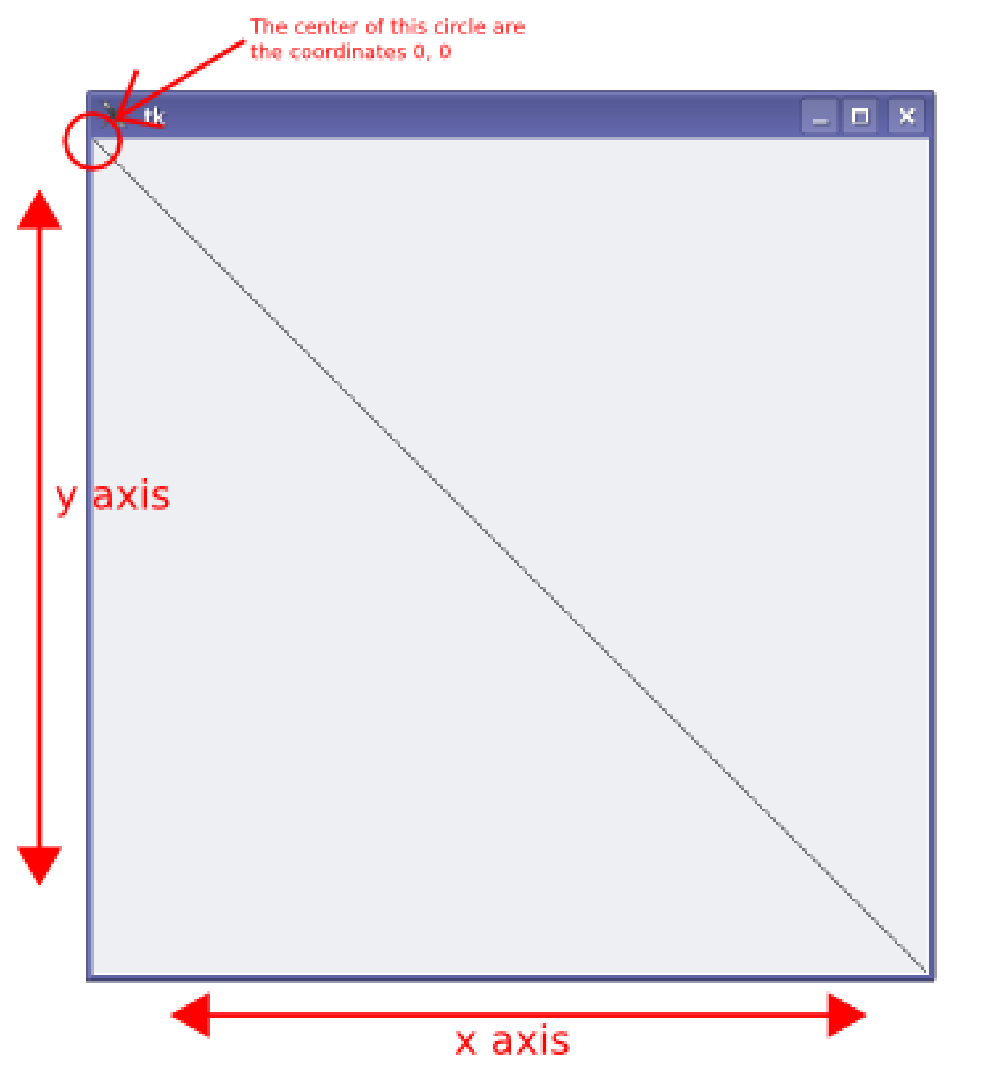
\includegraphics[width=80mm]{images/figure32}
%\end{center}
%\caption{Canvas x and y axis.}\label{fig32}
%\end{figure}
\begin{figure}
\begin{center}
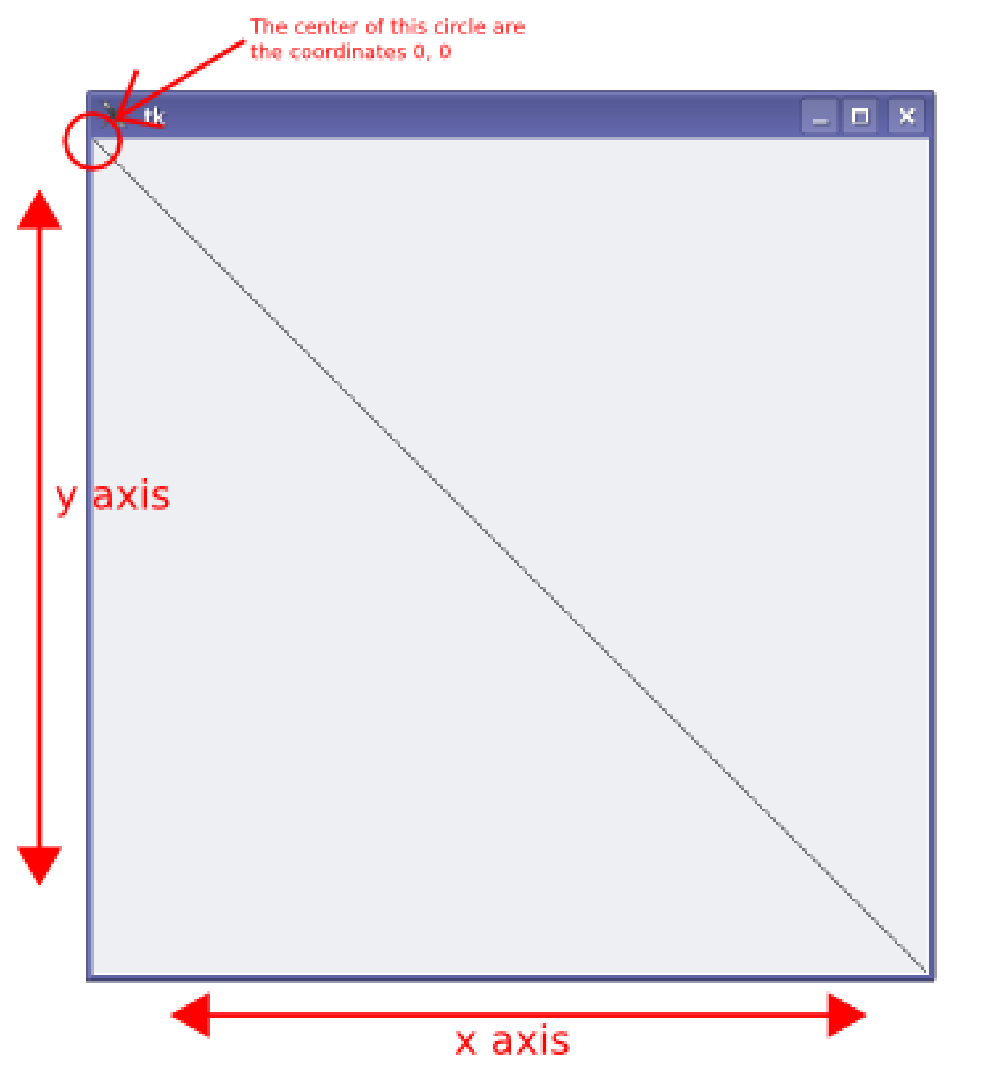
\includegraphics[width=80mm]{images/figure32}
\end{center}
\caption{Leinwand mit x- und y-Achse}\label{fig32}
\end{figure}

%Since the canvas is 500 pixels wide, and 500 pixels high, the coordinates of the bottom-right corner of the screen are 500,500. So the line in figure~\ref{fig32} can be drawn by using start coordinates of 0,0 and end coordinates of 500,500\index{modules!tkinter!create\_line}:
Nachdem die Leinwand 500 Pixel breit und 500 Pixel hoch ist, sind die Koordinaten der rechten unteren Ecke genau 500,500. Um also die Linie in Abbildung~\ref{fig32} zu zeichnen kannst du 0,0 als Startkoordinate und 500,500 als Zielkoordinate eingeben\index{Module!tkinter!create\_line}:

%\begin{Verbatim}[frame=single]
%>>> from tkinter import *
%>>> tk = Tk()
%>>> canvas = Canvas(tk, width=500, height=500)
%>>> canvas.pack()
%>>> canvas.create_line(0, 0, 500, 500)
%\end{Verbatim}
\begin{Verbatim}[frame=single]
>>> from tkinter import *
>>> tk = Tk()
>>> leinwand = Canvas(tk, width=500, height=500)
>>> leinwand.pack()
>>> leinwand.create_line(0, 0, 500, 500)
\end{Verbatim}

\noindent
%Now, to do the same thing with turtle, would have required the following code:
Hätte die Schildkröte diese Linie zeichnen sollen, hätte das so ausgeschaut:

%\begin{Verbatim}[frame=single]
%>>> import turtle
%>>> turtle.setup(width=500, height=500)
%>>> t = turtle.Pen()
%>>> t.up()
%>>> t.goto(-250,250)
%>>> t.down()
%>>> t.goto(500,-500)
%\end{Verbatim}
\begin{Verbatim}[frame=single]
>>> import turtle
>>> turtle.setup(width=500, height=500)
>>> stift = turtle.Pen()
>>> stift.up()
>>> stift.goto(-250,250)
>>> stift.down()
>>> stift.goto(500,-500)
\end{Verbatim}

%So the \code{tkinter} code is already an improvement, being shorter and less complicated. There are a large number of methods available on the canvas object, some of which aren't very useful to us, but let's take a look at some examples of the interesting functions.
Wie du siehst, ist der \code{tkinter}-Code schon eine Verbesserung, da er kürzer und einfacher ist. Und das canvas-Objekt hat auch sonst noch einige nützliche Methoden, die wir mit dem Leinwand-Objekt verwenden können.

%\section{Drawing Boxes}
\section{Rechtecke}

%In turtle, we drew a box by moving forward, turning, moving forward, turning again and so on. Eventually you can draw a rectangular or square box, just by changing how far you move forward. With tkinter, drawing a square or rectangle is considerably easier---you just need to know the coordinates for the corners.
Mit der Schildkröte haben wir Rechtecke und Quadrate gezeichnet, indem die Schildkröte immer eine Seite entlanggewandert ist, sich nach rechts umgedreht hat und die nächste Seite gezeichnet hat. Mit tkinter ist es viel einfacher ein Rechteck zu zeichnen---du brauchst nur die Koordinaten der Ecken zu kennen.


%\begin{Verbatim}[frame=single]
%>>> from tkinter import *
%>>> tk = Tk()
%>>> canvas = Canvas(tk, width=400,height=400)
%>>> canvas.pack()
%>>> canvas.create_rectangle(10, 10, 50, 50)
%1
%\end{Verbatim}
\begin{Verbatim}[frame=single]
>>> from tkinter import *
>>> tk = Tk()
>>> leinwand = Canvas(tk, width=400,height=400)
>>> leinwand.pack()
>>> leinwand.create_rectangle(10, 10, 50, 50)
1
\end{Verbatim}
%In the above example, we create a canvas that is 400 pixels wide, and 400 pixels high, and then we draw a square in the top left corner (the top left corner is 10 pixels in from the top left, and and the bottom right corner is 50 pixels in from the bottom right). You might be wondering what the number is that appeared when you typed \code{create\_rectangle}\index{modules!tkinter!create\_rectange} and earlier when calling \code{create\_line}?  That's an identifying number for the shape you've just drawn (whether a line or a square or a circle). We'll come back to that number later.
In diesem Beispiel erzeugen wir eine Leinwand, die 400 Pixel breit und 400 Pixel hoch ist. Danach zeichnen wir ein Quadrat im oberen linken Bereich. Du fragst dich vielleicht, was diese Nummer ist, die nach dem Zeichnen des Quadrates erschienen ist, als du \code{leinwand.create\_rectangle}\index{Module!tkinter!create\_rectange} eingegeben hast. Das ist die identifizierende Nummer für das eben gezeichnete Gebilde (egal, ob das eine Linie, ein Quadrat oder Kreis ist). Dazu kommen wir etwas später.

%The parameters that are passed to \code{create\_rectangle} are therefore: top left x position, top left y position, bottom right x position and bottom right y position. To save all that typing, we'll just refer to those as x1, y1 and x2, y2. We can draw a rectangle by making x2 a larger number:
Die Parameter, die du an \code{create\_rectangle} übergibst, sind folgende: linke obere x-Position und linke obere y-Position. Und danach die rechte untere x- und y-Position. Um uns diese Tipparbeit zu sparen werden wir ab jetzt x1, y1 für oben links und x2, y2 für unten rechts schreiben. Ein größeres Rechteck gibt es also wenn x2 größer wird.

%\begin{Verbatim}[frame=single]
%>>> canvas.create_rectangle(100, 100, 300, 50)
%\end{Verbatim}
\begin{Verbatim}[frame=single]
>>> leinwand.create_rectangle(100, 100, 300, 50)
\end{Verbatim}

\noindent
%Or by making y2 a bit larger:
Oder wenn y2 größer wird:

%\begin{Verbatim}[frame=single]
%>>> canvas.create_rectangle(100, 200, 150, 350)
%\end{Verbatim}
\begin{Verbatim}[frame=single]
>>> leinwand.create_rectangle(100, 200, 150, 350)
\end{Verbatim}

%That last rectangle is basically saying: go 100 pixels across the canvas (from the top left), and 200 pixels down, then draw a box across to 150 pixels and down to 350 pixels. At the moment you should have something like figure~\ref{fig33} on your canvas.
Mit diesem Beispiel sagt man Python soviel wie: gehe 100 Pixel nach rechts und 200 Pixel nach unten. Dann zeichne ein Rechteck, das 350 Pixel breit und 150 Pixel hoch ist. Nach allen Beispielen solltest du so etwas wie in Abbildung~\ref{fig33} sehen.

%\begin{figure}
%\begin{center}
%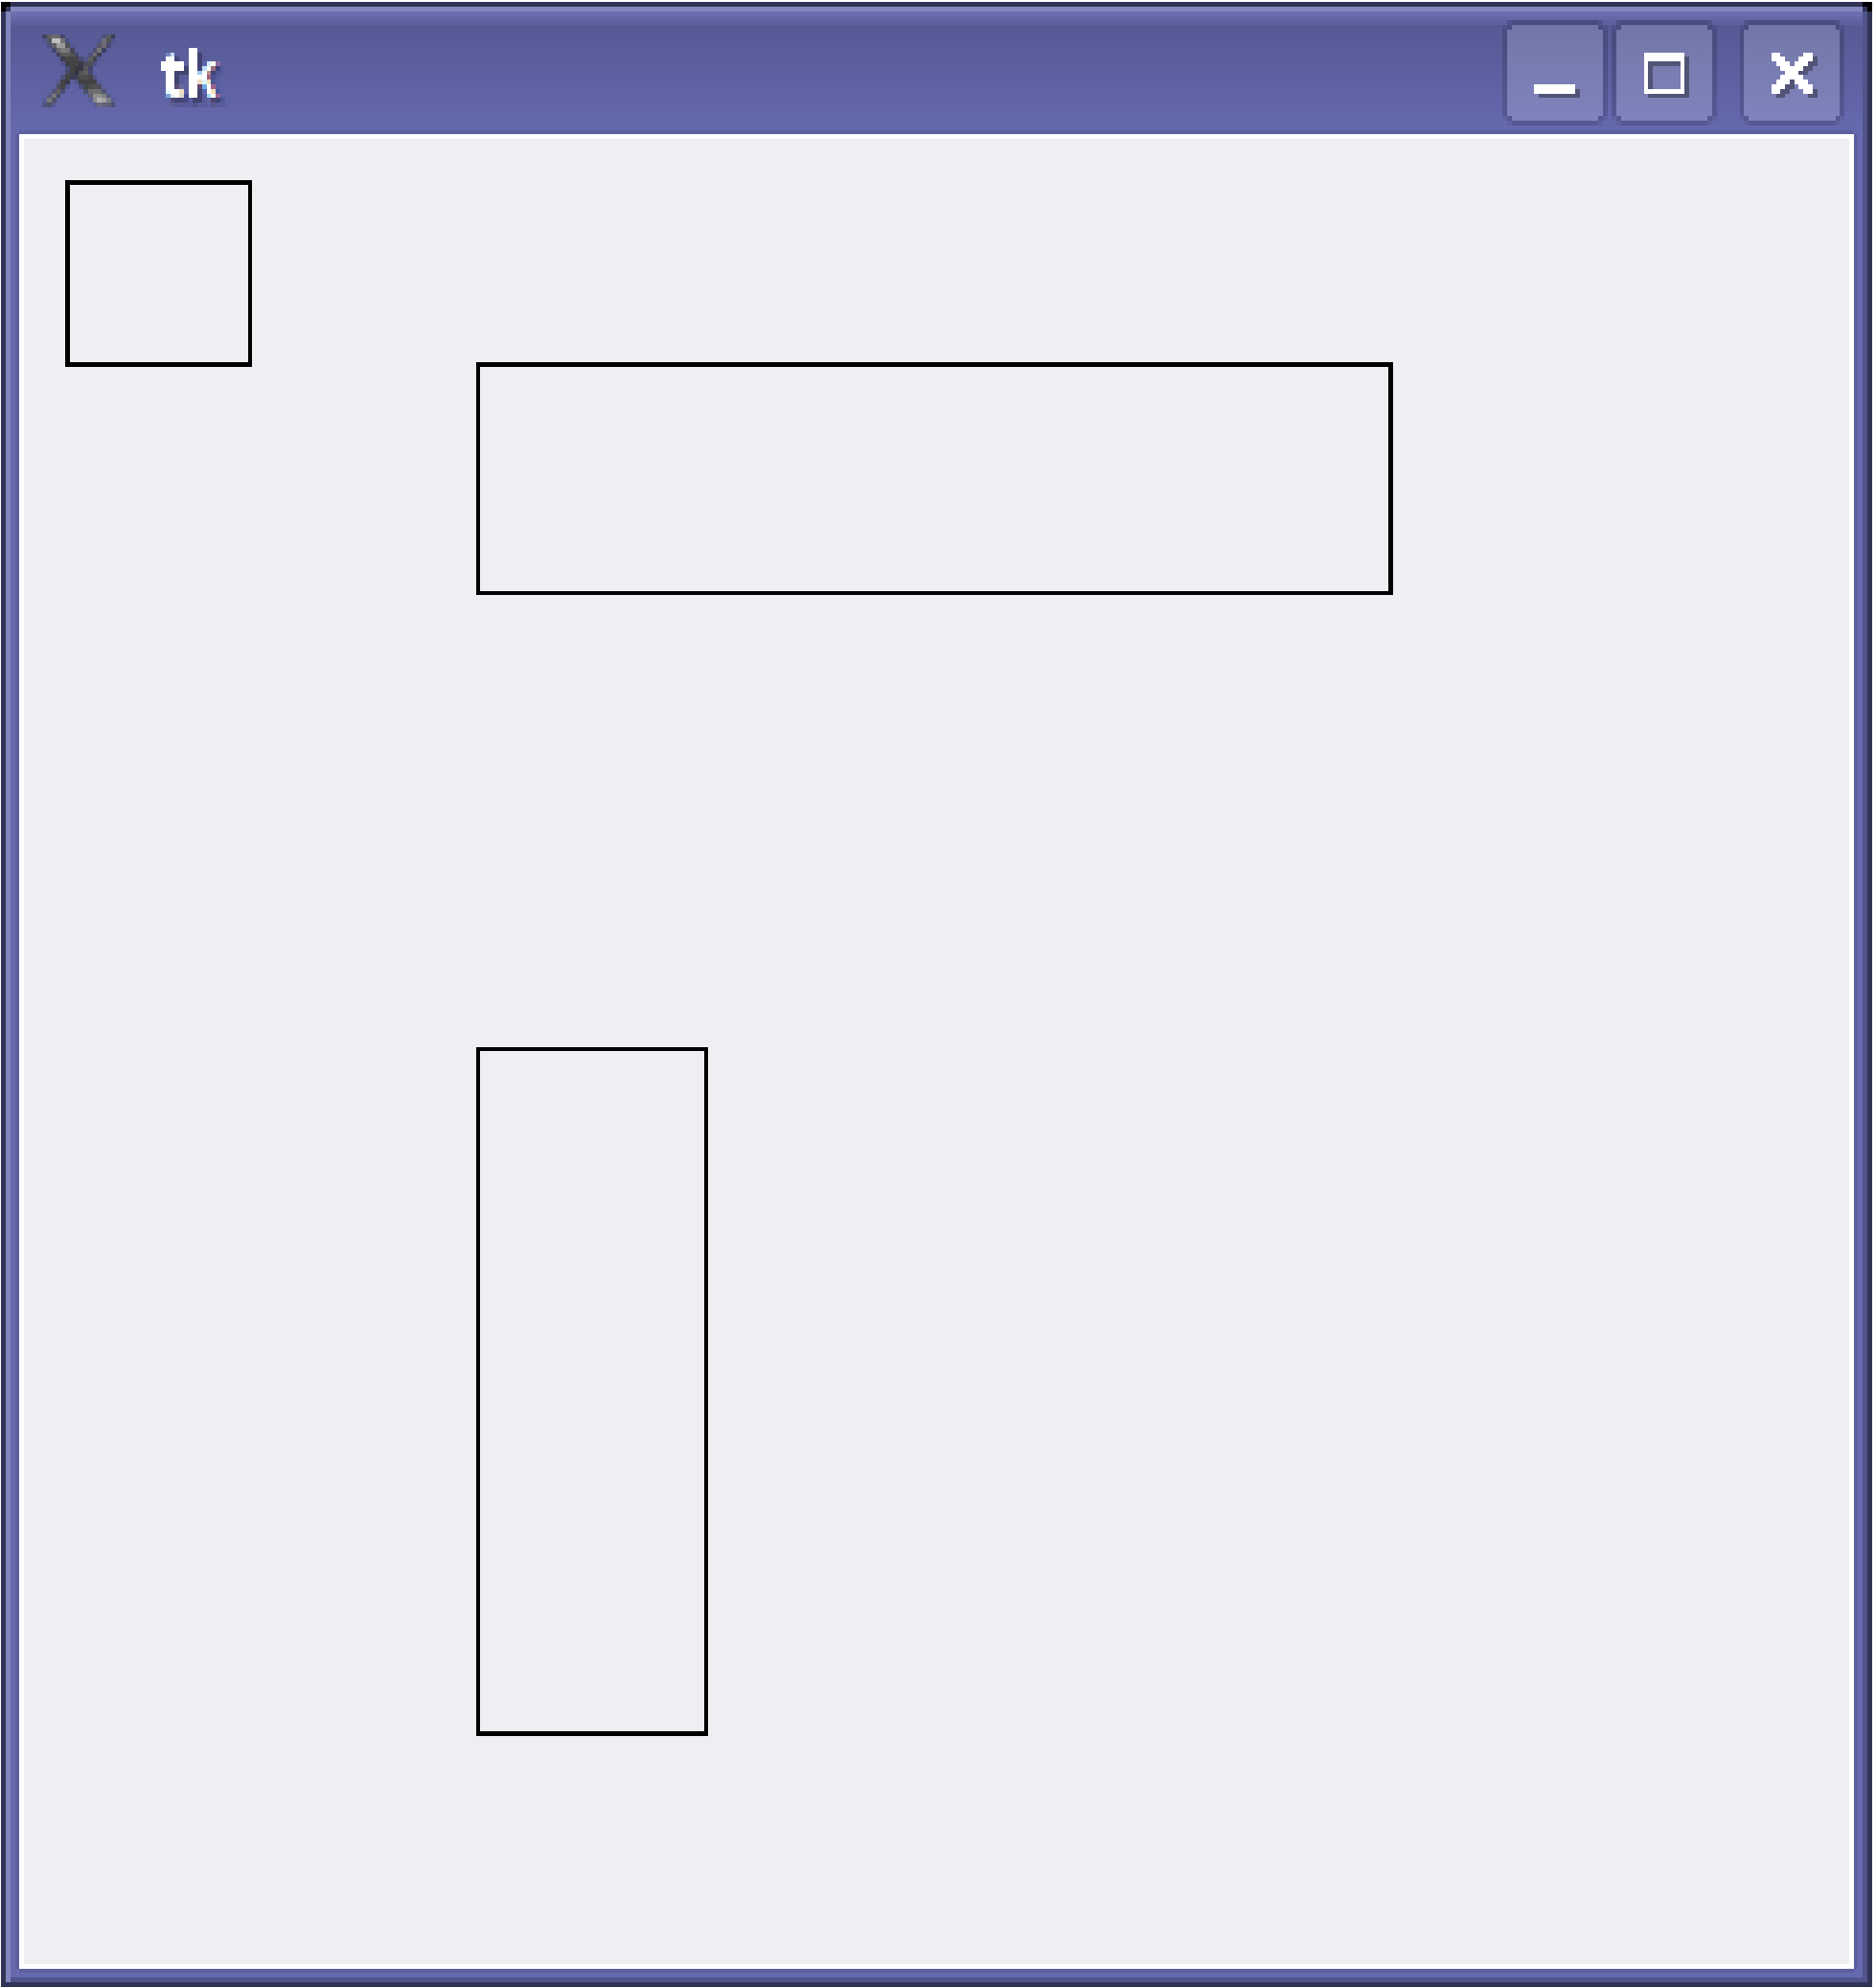
\includegraphics[width=80mm]{images/figure33}
%\end{center}
%\caption{tkinter boxes.}\label{fig33}
%\end{figure}
\begin{figure}
\begin{center}
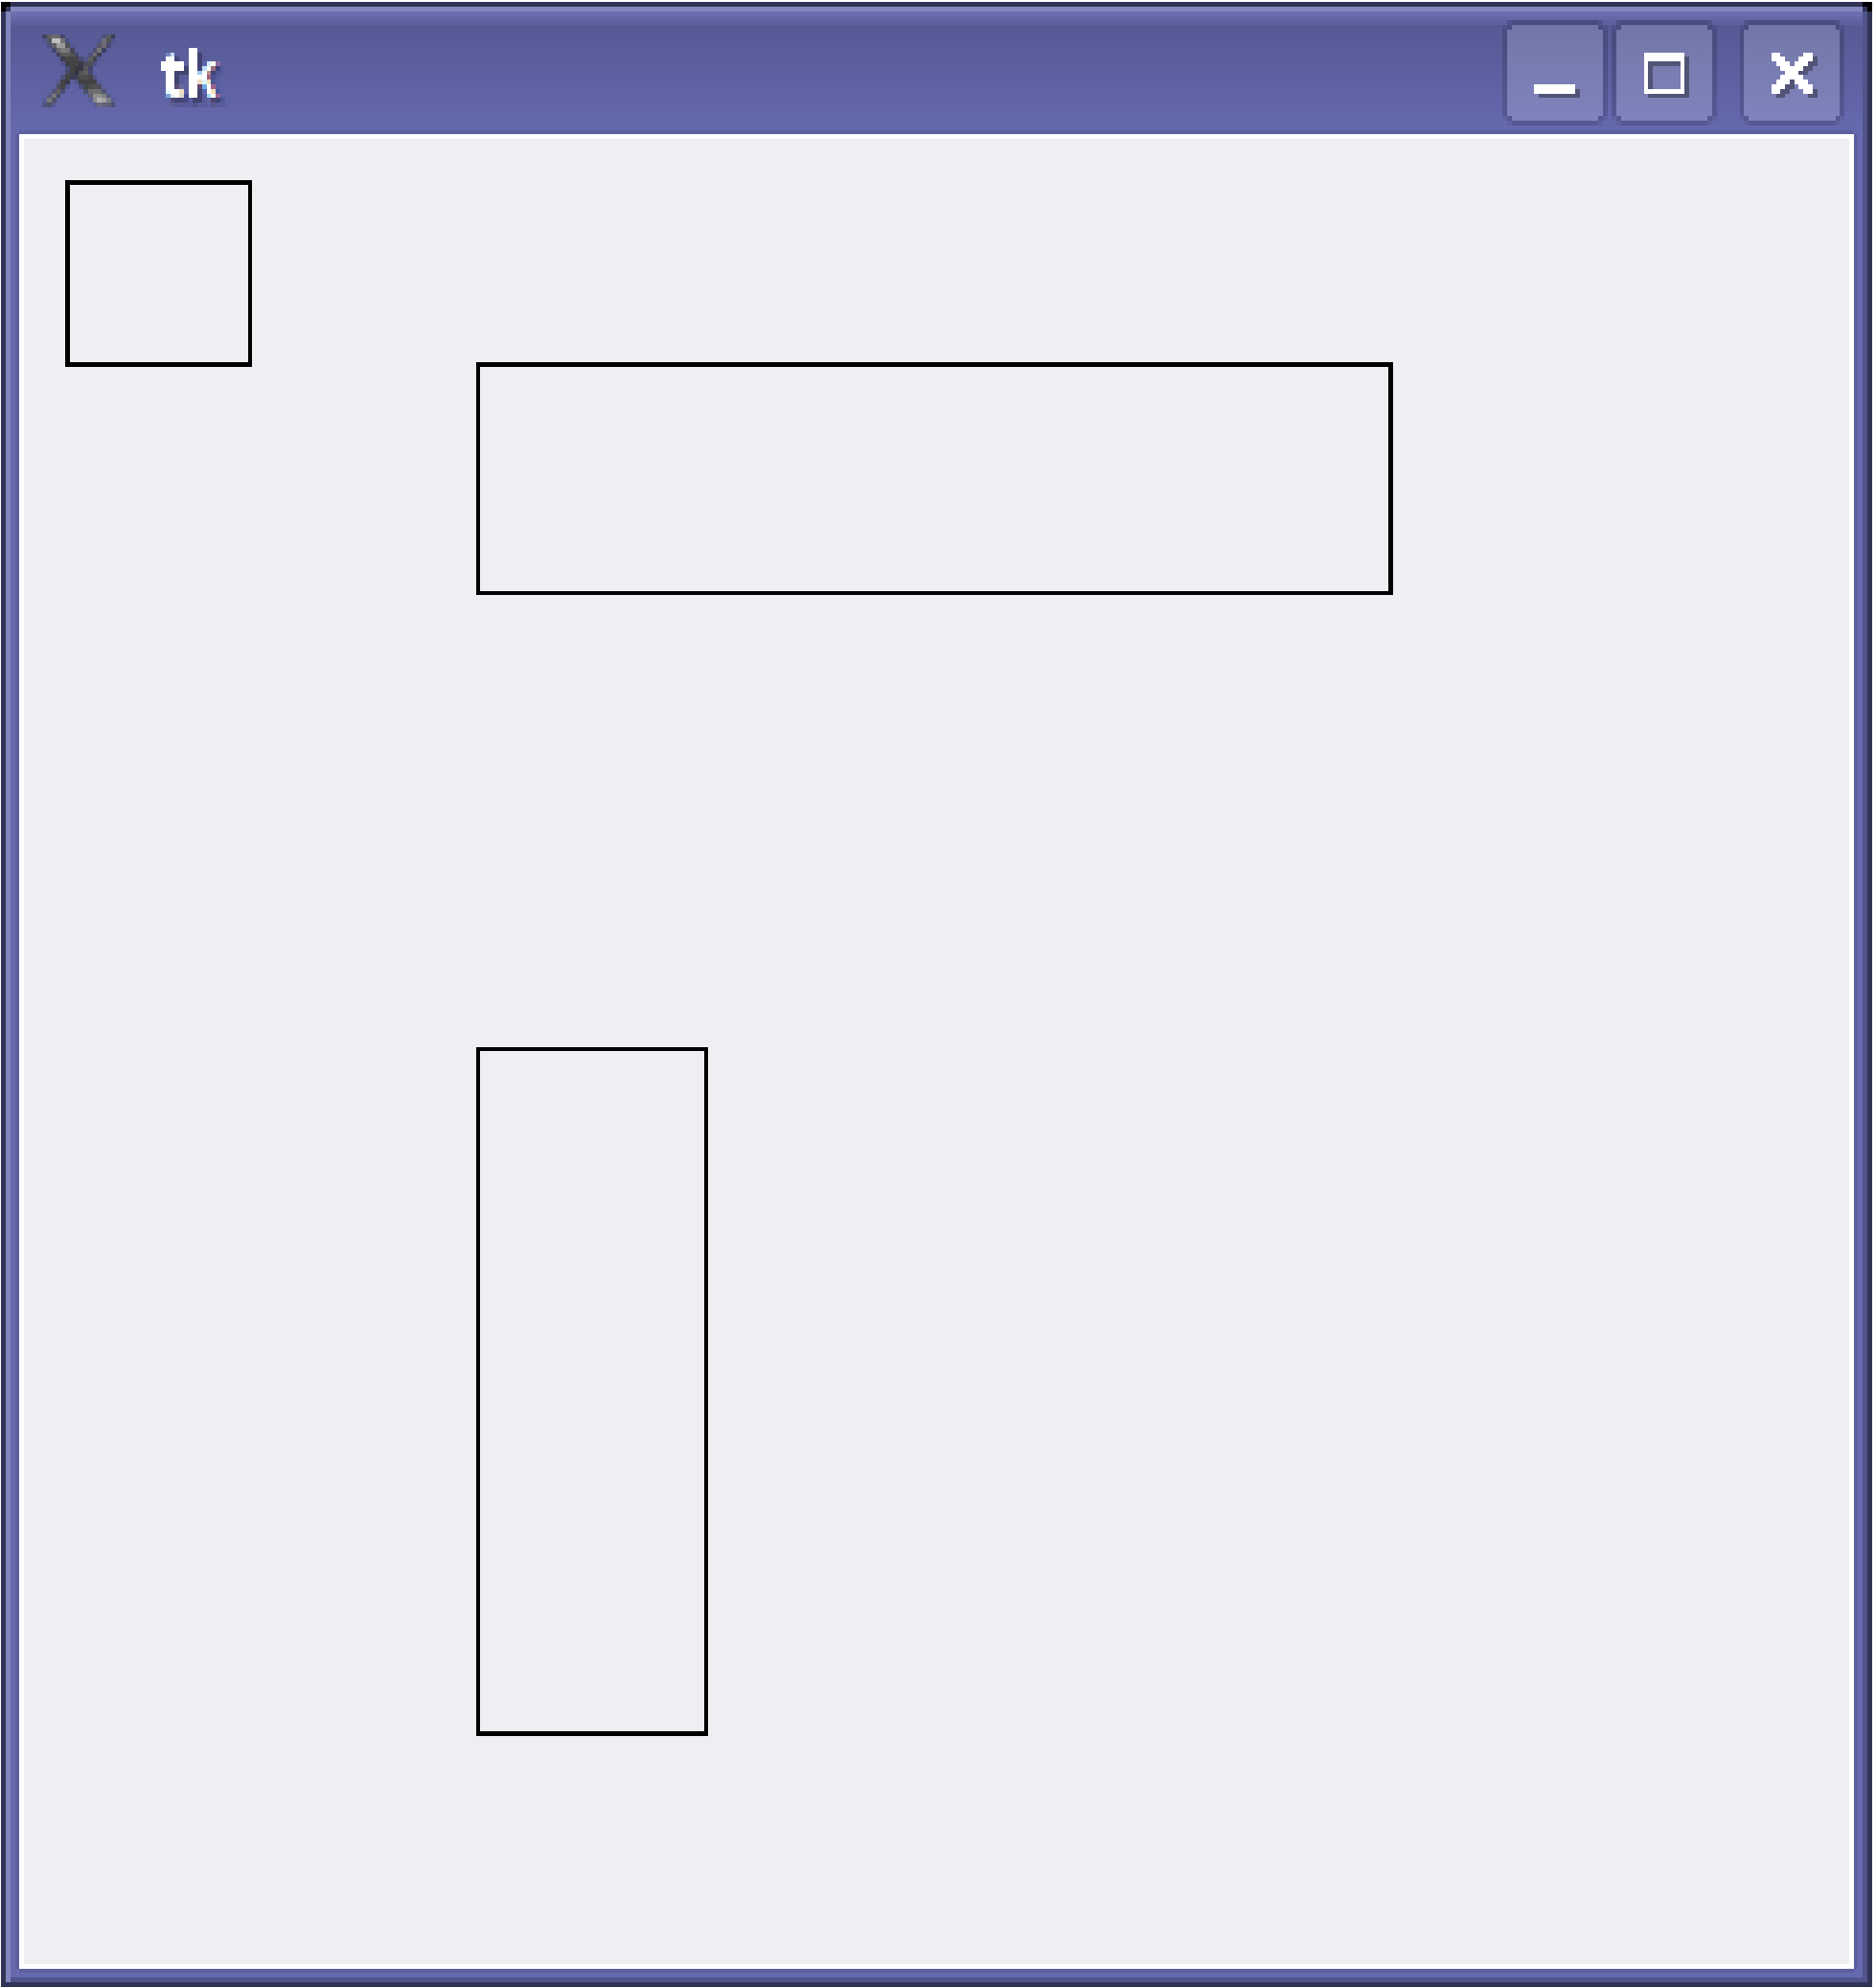
\includegraphics[width=80mm]{images/figure33}
\end{center}
\caption{Rechtecke mit tkinter gezeichnet.}\label{fig33}
\end{figure}

%Let's try filling the canvas with different sized rectangles. We can do this using a module called \code{random}\index{modules!random}. First import the random module:
Lass uns nun die Leinwand mit Rechtecken füllen, die alle eine eigene Farbe haben. Das können wir mit dem \code{random}\index{Module!random} machen. Zuerst importieren wir das Zufallsmodul (random):

%\begin{Verbatim}[frame=single]
%>>> import random
%\end{Verbatim}
\begin{Verbatim}[frame=single]
>>> import random
\end{Verbatim}

%Then we can create a function using a random number for the coordinates at the top and bottom corners. The function to use is called \code{randrange}\index{modules!random!randrange}:
Danach verwenden wir eine Funktion, die Zufallszahlen für die Koordinaten verwendet:

%\begin{Verbatim}[frame=single]
%>>> def random_rectangle(width, height):
%...     x1 = random.randrange(width)
%...     y1 = random.randrange(height)
%...     x2 = random.randrange(x1 + random.randrange(width))
%...     y2 = random.randrange(y1 + random.randrange(height))
%...     canvas.create_rectangle(x1, y1, x2, y2)
%\end{Verbatim}
\begin{Verbatim}[frame=single]
>>> def zufaelliges_rechteck(breite, hoehe):
...     x1 = random.randrange(breite)
...     y1 = random.randrange(hoehe)
...     x2 = random.randrange(x1 + random.randrange(breite))
...     y2 = random.randrange(y1 + random.randrange(hoehe))
...     leinwand.create_rectangle(x1, y1, x2, y2)
\end{Verbatim}

%In the first two lines we create variables for the top left corner of the rectangle using \code{randrange}, passing the width and the height.  The \code{randrange} function takes a number as an argument (actually, see Appendix~\ref{app:afewpythonmodules} for more uses of \code{randrange})---so \code{randrange(10)} gives you a number between 0 and 9, \code{randrange(100)} gives you a number between 0 and 99, and so on. The next two lines create variables for the bottom right corner of the rectangle (or square!)---we use the top left coordinate (x1 or y1) and add a random number to that variable. Finally we call the \code{create\_rectangle} function using those variables. You can try out the \code{random\_rectangle} function by passing the width and height of the canvas you created:
In den ersten zwei Zeilen erzeugen wir Zufallsvariablen für die x- und y-Koordinaten der oberen linken Ecke. Die \code{randrange}-Funktion schränkt die Zahlen ein die zurückkommen können. Ein \code{randrang(10)} gibt zum Beispiel die Zahlen zwischen 0 und 9 zurück. Die nächsten zwei Zeilen erzeugen Variablen für die Koordinaten der rechten unteren Ecke. Zu guter Letzt wird mit der \code{random\_rectangle} Funktion das Rechteck auf der Leinwand gezeichnet.

%\begin{Verbatim}[frame=single]
%>>> random_rectangle(400, 400)
%\end{Verbatim}
\begin{Verbatim}[frame=single]
>>> zufaelliges_rechteck(400, 400)
\end{Verbatim}

\noindent
%Or to fill the screen, how about creating a loop to call it a number of times:
Oder gleich eine Menge von Rechtecken in einer Schleife erzeugen:

%\begin{Verbatim}[frame=single]
%>>> for x in range(0, 100):
%...     random_rectangle(400, 400)
%\end{Verbatim}
\begin{Verbatim}[frame=single]
>>> for x in range(0, 100):
...     zufaelliges_rechteck(400, 400)
\end{Verbatim}

\noindent
%Which produces a bit of a mess (figure~\ref{fig34}, but is interesting nonetheless.
Da kommt zwar eine große Unordnung raus (Abbildung~\ref{fig34}), aber das ist trotzdem interessant.

%\begin{figure}
%\begin{center}
%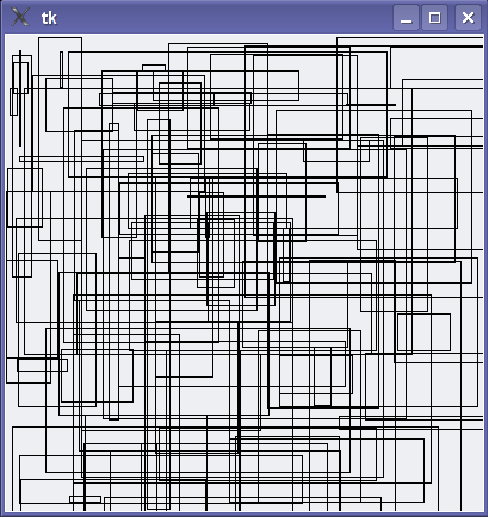
\includegraphics[width=80mm]{images/figure34}
%\end{center}
%\caption{A mess of rectangles.}\label{fig34}
%\end{figure}
\begin{figure}
\begin{center}
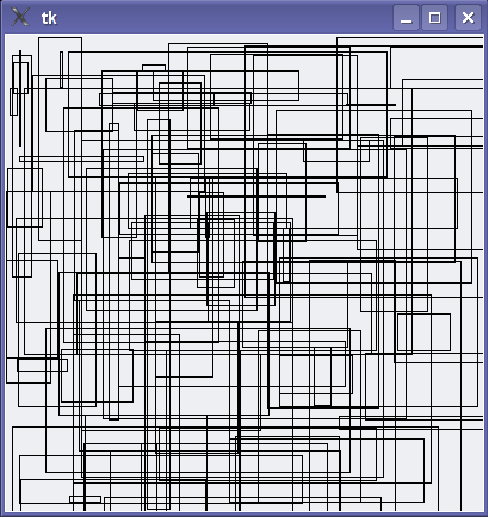
\includegraphics[width=80mm]{images/figure34}
\end{center}
\caption{Rechtecke, wohin man schaut.}\label{fig34}
\end{figure}

%Remember, back in the last chapter, we set the colour the turtle drew with using percentages of the 3 colours: red, green and blue? With \code{tkinter} you can set the colour using similar ideas, but unfortunately, it's slightly more complicated than with \code{turtle}.  First of all, let's change the random rectangle function to pass in a colour to fill the rectangle with:
Im letzten Kapitel haben wir die Schildkröte Linien in verschiedenen Farben zeichnen lassen. Das waren die Grundfarben rot, grün und blau. Mit \code{tkinter} kannst du auch Farben verwenden. Es ist aber ein wenig komplizierter. Lass uns zuerst unsere Funktion zum Reckteck Zeichnen anpassen, damit wir auch eine Farbe mitgeben können:

%\begin{Verbatim}[frame=single]
%>>> def random_rectangle(width, height, fill_colour):
%...     x1 = random.randrange(width)
%...     y1 = random.randrange(height)
%...     x2 = random.randrange(x1 + random.randrange(width))
%...     y2 = random.randrange(y1 + random.randrange(height))
%...     canvas.create_rectangle(x1, y1, x2, y2, fill=fill_colour)
%\end{Verbatim}
\begin{Verbatim}[frame=single]
>>> def zufaelliges_rechteck(breite, hoehe, farbe):
...     x1 = random.randrange(breite)
...     y1 = random.randrange(hoehe)
...     x2 = random.randrange(x1 + random.randrange(breite))
...     y2 = random.randrange(y1 + random.randrange(hoehe))
...     leinwand.create_rectangle(x1, y1, x2, y2, fill=farbe)
\end{Verbatim}

%The canvas \code{create\_rectangle} function can take a parameter `fill' which specifies the fill colour.  We can now pass this into the function. Try the following:
Jetzt können wir der \code{create\_rectangle} Funktion auch den Farbparameter `fill' mitgeben. Probiere Folgendes aus:

%\begin{Verbatim}[frame=single]
%>>> random_rectangle(400, 400, 'green')
%>>> random_rectangle(400, 400, 'red')
%>>> random_rectangle(400, 400, 'blue')
%>>> random_rectangle(400, 400, 'orange')
%>>> random_rectangle(400, 400, 'yellow')
%>>> random_rectangle(400, 400, 'pink')
%>>> random_rectangle(400, 400, 'purple')
%>>> random_rectangle(400, 400, 'violet')
%>>> random_rectangle(400, 400, 'magenta')
%>>> random_rectangle(400, 400, 'cyan')
%\end{Verbatim}
\begin{Verbatim}[frame=single]
>>> zufaelliges_rechteck(400, 400, 'green')
>>> zufaelliges_rechteck(400, 400, 'red')
>>> zufaelliges_rechteck(400, 400, 'blue')
>>> zufaelliges_rechteck(400, 400, 'orange')
>>> zufaelliges_rechteck(400, 400, 'yellow')
>>> zufaelliges_rechteck(400, 400, 'pink')
>>> zufaelliges_rechteck(400, 400, 'purple')
>>> zufaelliges_rechteck(400, 400, 'violet')
>>> zufaelliges_rechteck(400, 400, 'magenta')
>>> zufaelliges_rechteck(400, 400, 'cyan')
\end{Verbatim}

%Some, and maybe all, of those named colours will work.  But some of them might result in an error message (it depends on whether you're using Windows, Mac OS X or Linux). So far, that's pretty easy.  But what about a colour like gold?  In the \code{turtle} module, we created gold using 100\% of red, 85\% of green and no blue.  In \code{tkinter} we can create gold using:
Die meisten Farben müssten so funktionieren. Aber manche könnten auch eine Fehlermeldung zurückgeben, je nachdem, ob du Windows, Mac OS X oder Linux verwendest. So weit, so gut. Aber was ist mit der goldenen Farbe? Mit der Schildkröte haben wir Gold aus 100\% Rot und 85\% Grün erzeugt. Mit \code{tkinter} könnten wir Gold folgendermaßen erzeugen:

%\begin{Verbatim}[frame=single]
%>>> random_rectangle(400, 400, '#ffd800')
%\end{Verbatim}
\begin{Verbatim}[frame=single]
>>> zufaelliges_rechteck(400, 400, '#ffd800')
\end{Verbatim}

%Which, all in all, is a pretty strange way to create a colour.  `ffd800' is called hexadecimal\index{hexadecimal colors}, and is another way to represent numbers.  Explaining how hexadecimal numbers work would take a few more pages than we have to spare for this book, so for the moment, you can use the following function to create a hexadecimal colour:
Was natürlich eine komische Art ist um Farben zu erzeugen. `ffd800' ist eine Hexadezimalzahl\index{hexadezimale Zahlen} und eine andere Art um Zahlen auszudrücken. Die Erklärung von Hexadezimalzahlen würde jetzt zu weit führen, aber in der Zwischenzeit kannst du folgende Funktion verwenden um hexadezimale Zahlen zu erzeugen:

%\begin{Verbatim}[frame=single]
%>>> def hexcolor(red, green, blue):
%...     red = 255*(red/100.0)
%...     green = 255*(green/100.0)
%...     blue = 255*(blue/100.0)
%...     return '#%02x%02x%02x' % (red, green, blue)
%\end{Verbatim}
\begin{Verbatim}[frame=single]
>>> def hexfarbe(rot, gruen, blau):
...     rot = 255*(rot/100.0)
...     gruen = 255*(gruen/100.0)
...     blau = 255*(blau/100.0)
...     return '#%02x%02x%02x' % (rot, gruen, blau)
\end{Verbatim}

%Calling hexcolor with 100\% for red, 85\% for green and 0\% for blue, results in the hexadecimal for a gold colour we just used:
Die hexfarbe-Funktion mit 100\% Rot, 85\% grün und 0\% Blau aufzurufen, gibt den hexadezimalen Wert für die Farbe Gold zurück:

%\begin{Verbatim}[frame=single]
%>>> print(hexcolor(100, 85, 0))
%#ffd800
%\end{Verbatim}
\begin{Verbatim}[frame=single]
>>> print(hexfarbe(100, 85, 0))
#ffd800
\end{Verbatim}

\noindent
%You can create a bright purple colour using 98\% of red, 1\% of green, and 77\% of blue:
Und ein helles Lila aus 98\% Rot, 1\% Rot und 77\% blau ist:

%\begin{Verbatim}[frame=single]
%>>> print(hexcolor(98, 1, 77))
%#f902c4
%\end{Verbatim}
\begin{Verbatim}[frame=single]
>>> print(hexfarbe(98, 1, 77))
#f902c4
\end{Verbatim}

\noindent
%You can use that with the random\_rectangle function we created earlier:
Du kannst das auch mit der zufaelliges\_rechteck Funktion von vorher kombinieren:

%\begin{Verbatim}[frame=single]
%>>> random_rectangle(400, 400, hexcolor(98, 1, 77))
%\end{Verbatim}
\begin{Verbatim}[frame=single]
>>> zufaelliges_rechteck(400, 400, hexfarbe(98, 1, 77))
\end{Verbatim}

%\begin{figure}
%\begin{center}
%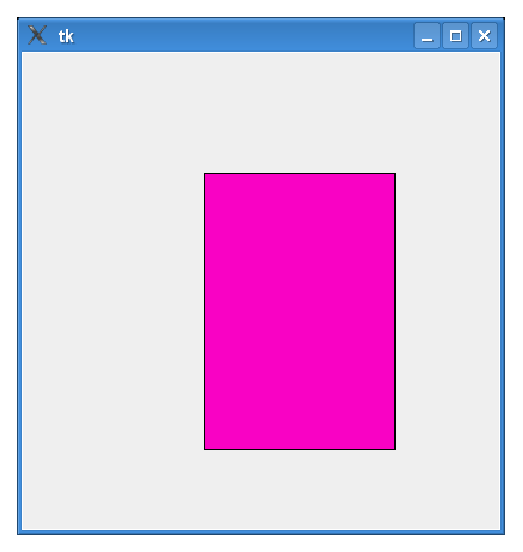
\includegraphics[width=80mm]{images/figure35}
%\end{center}
%\caption{A purple rectangle.}\label{fig35}
%\end{figure}
\begin{figure}
\begin{center}
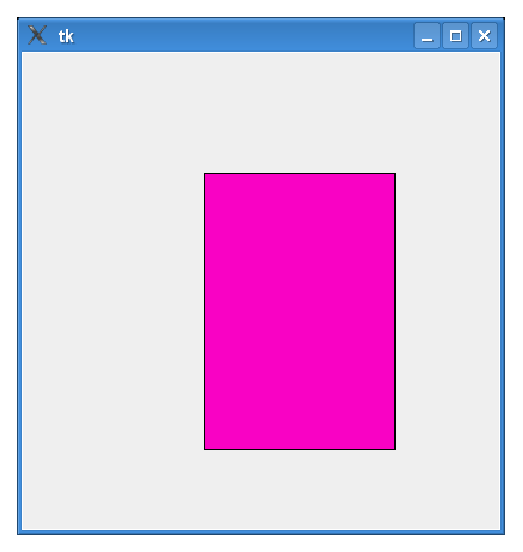
\includegraphics[width=80mm]{images/figure35}
\end{center}
\caption{Ein pinkes Rechteck.}\label{fig35}
\end{figure}

%\section{Drawing Arcs}
\section{Bögen}

%An arc is a part of a circle, but to draw one with tkinter you need to draw a rectangle. Which doesn't make a lot of sense until you try to draw a rectangle and then draw an arc inside it (see figure~\ref{fig36}). The code to draw this arc might look something like this\index{modules!tkinter!create\_arc}:
Um mit tkinter einen Bogen zu zeichnen, fängt man mit einem Rechteck an. Und in dieses Rechteck wird dann der Bogen reingezeichnet (siehe Abbildung~\ref{fig36}). Der Code dazu könnte so ausschauen\index{Module!tkinter!create\_arc}:

%\begin{Verbatim}[frame=single]
%canvas.create_arc(10, 10, 200, 100, extent=180, style=ARC)
%\end{Verbatim}
\begin{Verbatim}[frame=single]
leinwand.create_arc(10, 10, 200, 100, extent=180, style=ARC)
\end{Verbatim}

%\begin{figure}
%\begin{center}
%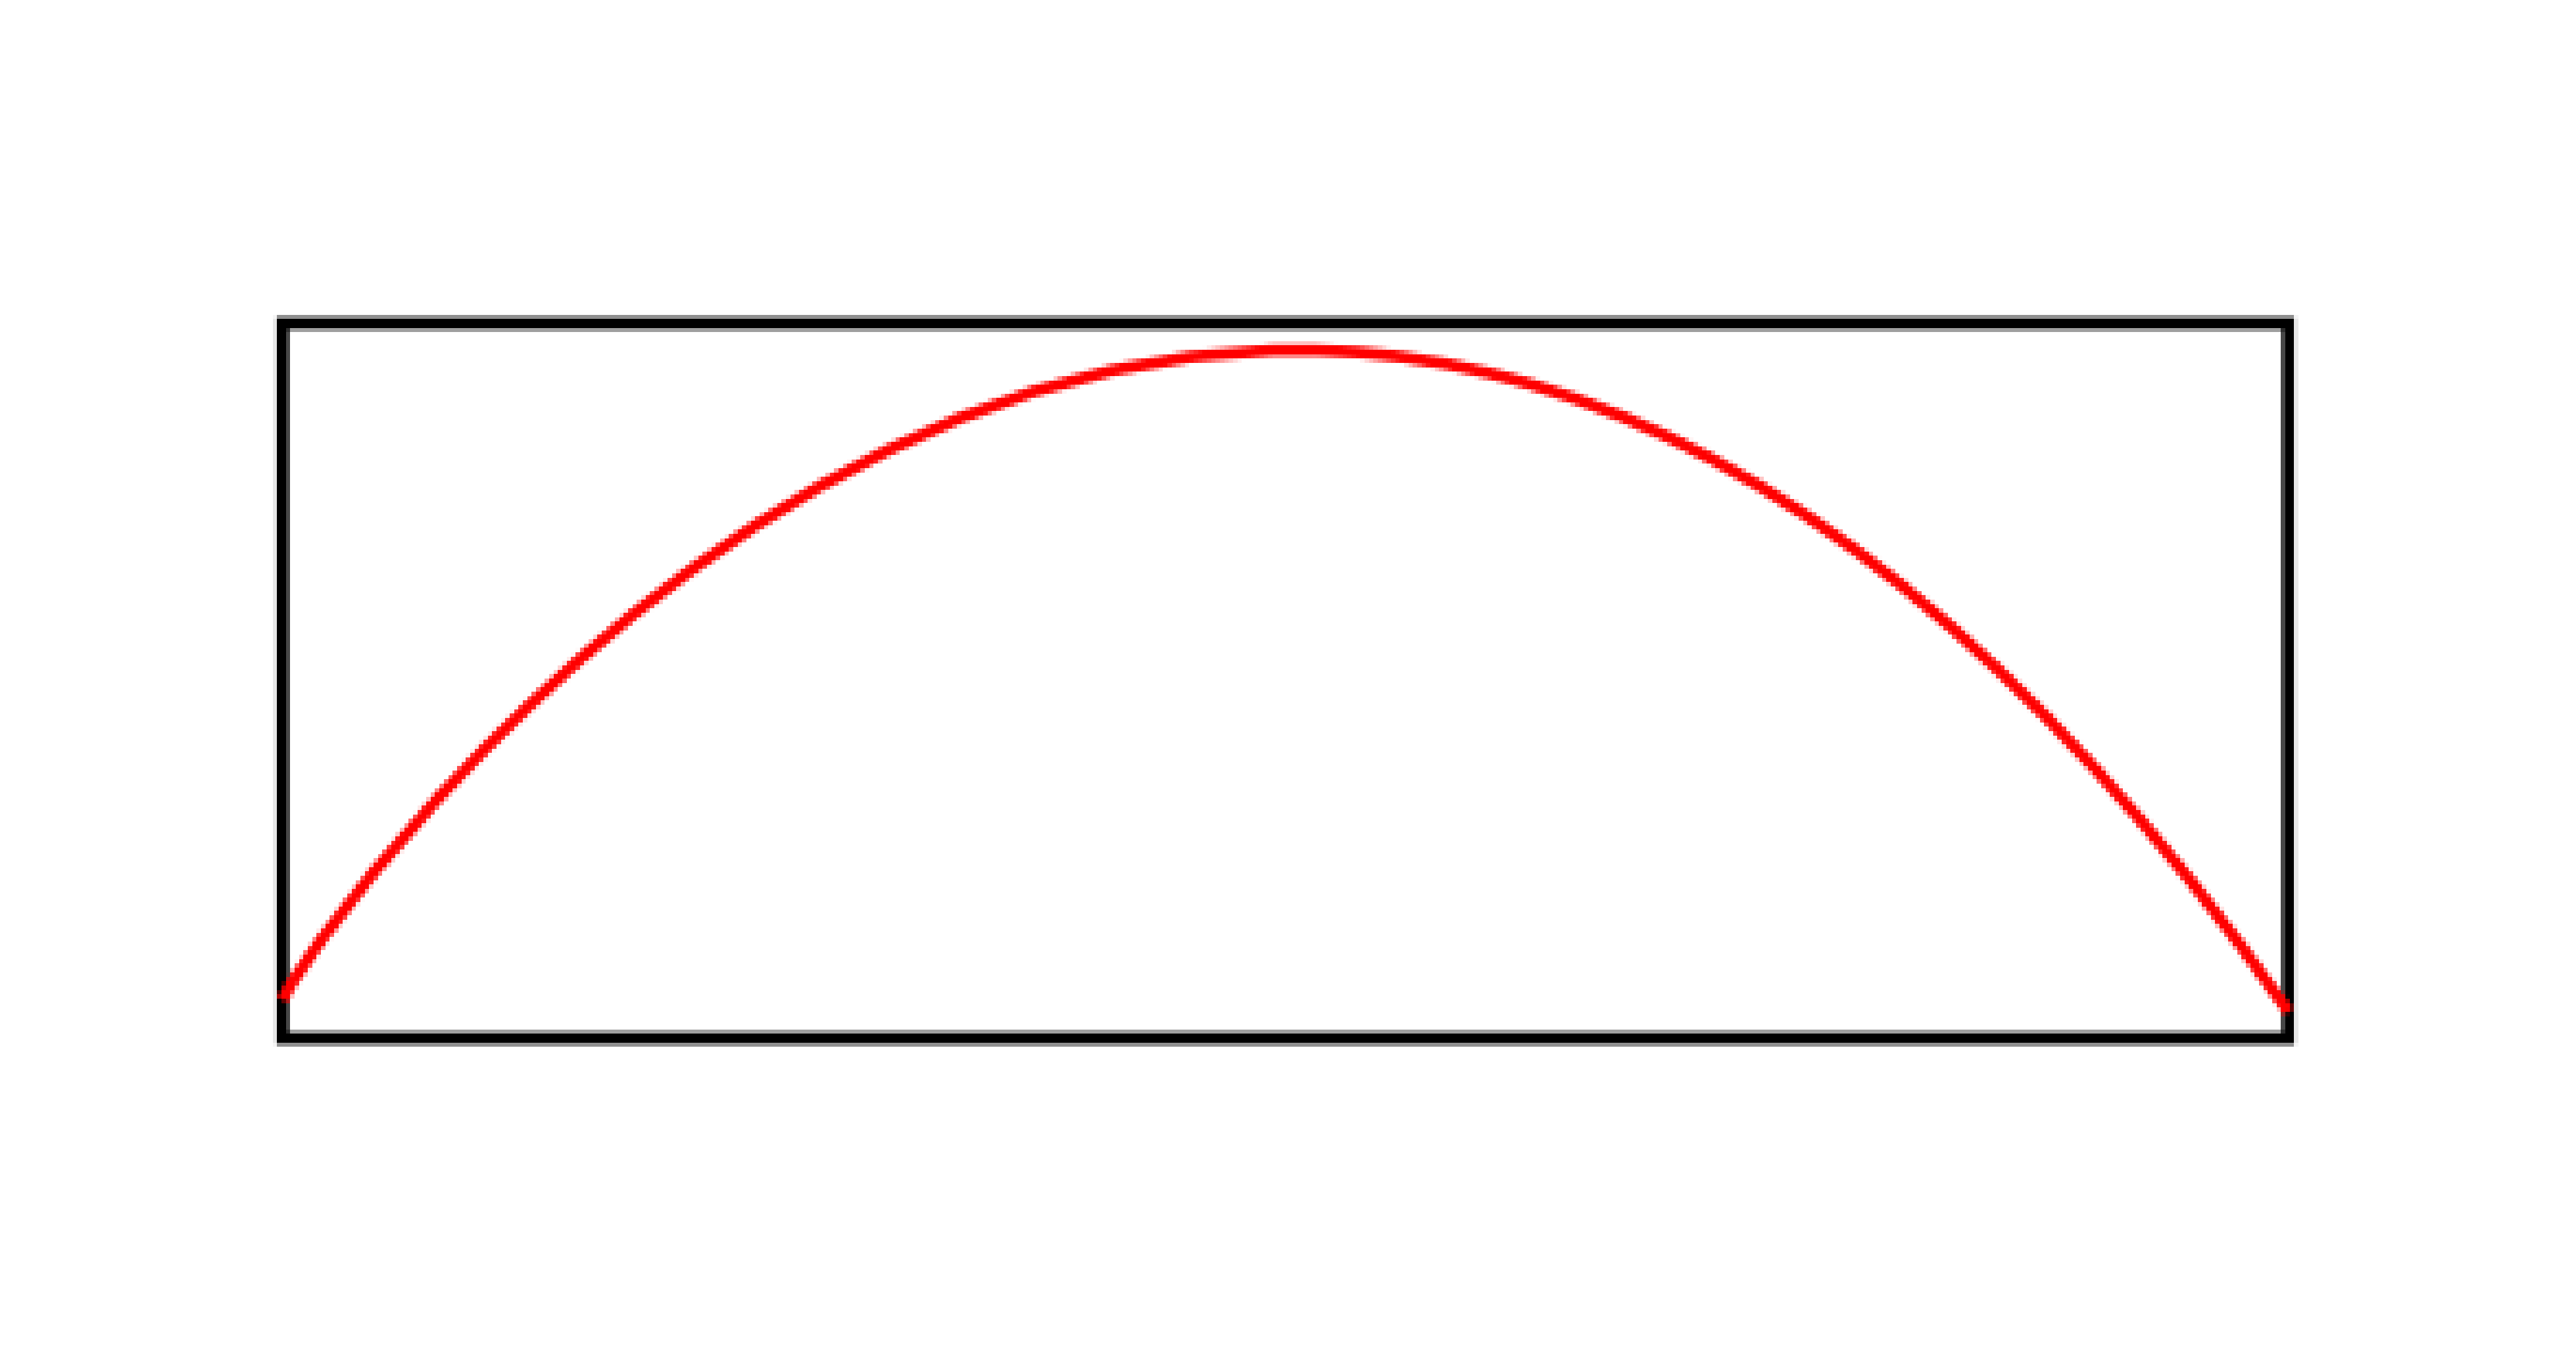
\includegraphics[width=80mm]{images/figure36}
%\end{center}
%\caption{An arc fitting inside a rectangle.}\label{fig36}
%\end{figure}
\begin{figure}
\begin{center}
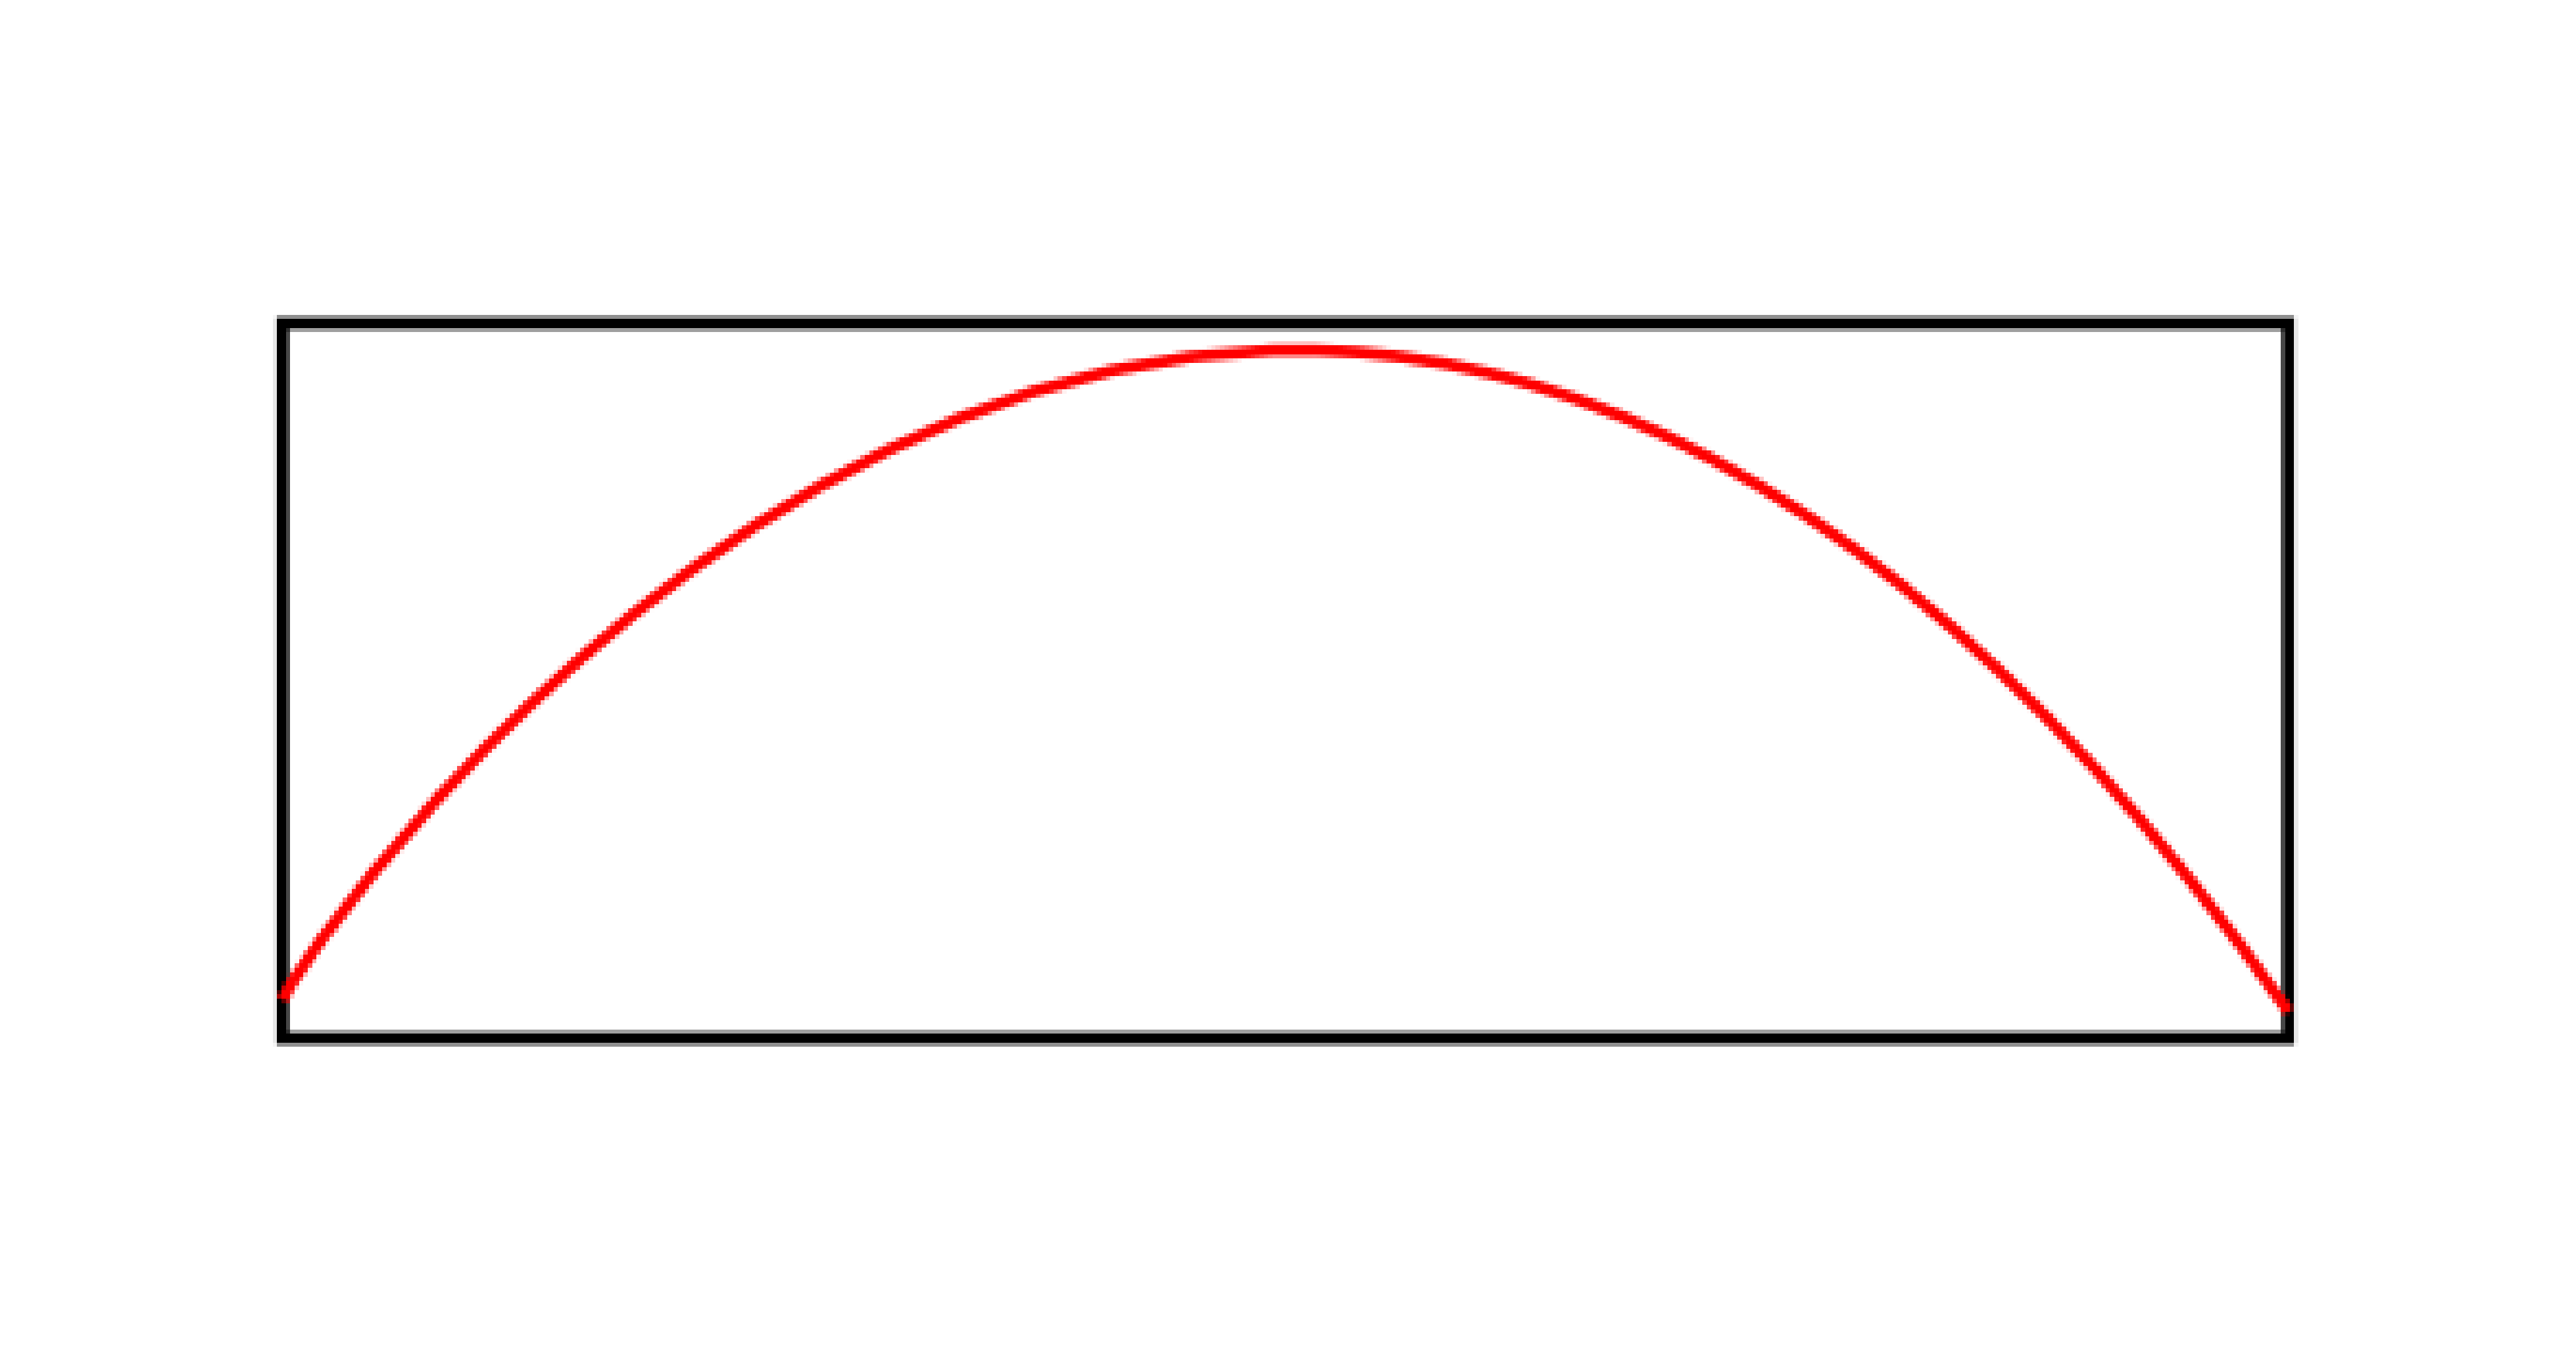
\includegraphics[width=80mm]{images/figure36}
\end{center}
\caption{Ein Bogen innerhalb eines Rechtecks.}\label{fig36}
\end{figure}

%This places the top left corner of the rectangle at the coordinates 10, 10 (that's 10 pixels across, 10 pixels down), and the bottom right corner of the rectangle at the coordinates 200, 100 (200 pixels across, 100 pixels down).  The next parameter (a \textbf{named} parameter) `extent' is used to specify the degrees of the angle of the arc.  If you don't know anything about degrees in a circle (or arc), then just remember that if you think about a circle, 180 degrees would be half of the circle (or half the arc), 359 degrees would be a full circle, 90 degrees is a quarter of a circle and 0 degrees is\texorpdfstring{$\ldots$}{...} well, nothing at all. Here's some code that draws a bunch of different arcs down the page so you can see the basic differences when we use different degrees (you can see the examples in figure~\ref{fig37}):
Somit ist die obere linke Ecke auf den Koordinaten 10, 10 (also 10 nach rechts und 10 nach unten) und die rechte untere Ecke auf den Koordinaten 200, 100 (200 nach rechts und 100 nach unten). Der nächste Parameter (ein \textbf{benannter} Parameter), `extend', wird benutzt um den Kreis näher in Grad zu beschreiben. Dabei entsprechen 359 Grad einem vollen Kreis und 180 einem halben. Probiere die nächsten Zeilen aus, um zu sehen, wie sich die Parameter auswirken (das Ergebnis siehst du in Abbildung~\ref{fig37}):

%\begin{Verbatim}[frame=single]
%>>> canvas.create_arc(10, 10, 200, 80, extent=45, style=ARC)
%>>> canvas.create_arc(10, 80, 200, 160, extent=90, style=ARC)
%>>> canvas.create_arc(10, 160, 200, 240, extent=135, style=ARC)
%>>> canvas.create_arc(10, 240, 200, 320, extent=180, style=ARC)
%>>> canvas.create_arc(10, 320, 200, 400, extent=359, style=ARC)
%\end{Verbatim}
\begin{Verbatim}[frame=single]
>>> leinwand.create_arc(10,  10, 200,  80, extent= 45, style=ARC)
>>> leinwand.create_arc(10,  80, 200, 160, extent= 90, style=ARC)
>>> leinwand.create_arc(10, 160, 200, 240, extent=135, style=ARC)
>>> leinwand.create_arc(10, 240, 200, 320, extent=180, style=ARC)
>>> leinwand.create_arc(10, 320, 200, 400, extent=359, style=ARC)
\end{Verbatim}

%\begin{figure}
%\begin{center}
%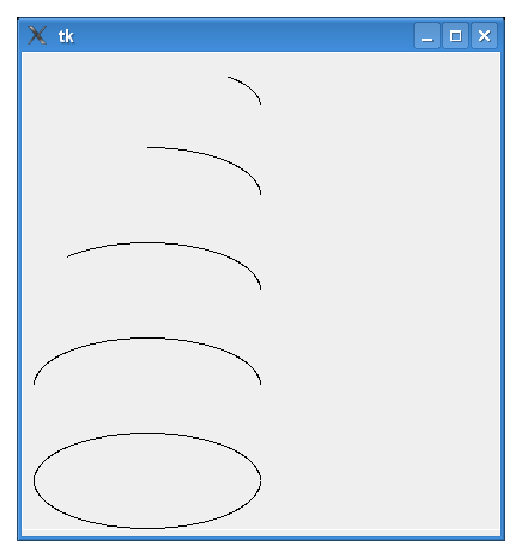
\includegraphics[width=80mm]{images/figure37}
%\end{center}
%\caption{Differing degrees of arcs.}\label{fig37}
%\end{figure}
\begin{figure}
\begin{center}
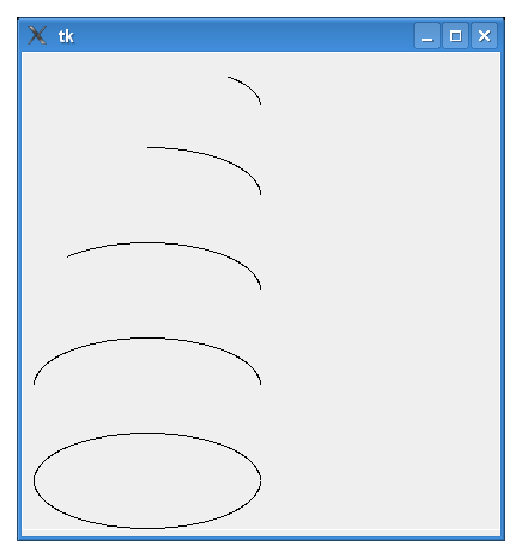
\includegraphics[width=80mm]{images/figure37}
\end{center}
\caption{Verschiedene Varianten von Bögen.}\label{fig37}
\end{figure}

%\section{Drawing Ovals}
\section{Ellipsen}

%While the last statement in the above example draws an oval, you can also draw ovals using the \code{create\_oval}\index{modules!tkinter!create\_oval} function.  Similar to drawing arcs, an oval is drawn inside the boundaries of a rectangle. For example, the following code:
Mit dem letzten Befehl des vorigen Abschnitts kommt schon ein ovaler Kreis (eine Ellipse) raus. Aber auch die Funktion \code{create\_oval}\index{Module!tkinter!create\_oval} erzeugt eine Ellipse. Ähnlich zu den Bögen, wird der ovale Kreis innerhalb eines Rechtecks gezeichnet. Zum Beispiel mit folgendem Code:

%\begin{Verbatim}[frame=single]
%>>> tk = Tk()
%>>> canvas = Canvas(tk, width=400,height=400)
%>>> canvas.pack()
%>>> canvas.create_oval(1, 1, 300, 200)
%\end{Verbatim}
\begin{Verbatim}[frame=single]
>>> tk = Tk()
>>> leinwand = Canvas(tk, width=400,height=400)
>>> leinwand.pack()
>>> leinwand.create_oval(1, 1, 300, 200)
\end{Verbatim}

%This example draws an oval in the (imaginary) square drawn from pixel positions 1,1 to 300,200. If we draw a red rectangle with the same coordinates, you can properly see how the oval is drawn inside (figure~\ref{fig38}):
Dieser Code zeichnet die Ellipse ins imaginäre Rechteck mit den Eckpunkten 1,1 und 300,200. Zum verdeutlischen kannst du noch ein rotes Rechteck herum zeichnen (siehe Abbildung~\ref{fig39}):

%\begin{Verbatim}[frame=single]
%>>> canvas.create_rectangle(1, 1, 300, 200, outline="#ff0000")
%\end{Verbatim}
\begin{Verbatim}[frame=single]
>>> leinwand.create_rectangle(1, 1, 300, 200, outline="#ff0000")
\end{Verbatim}

%\begin{figure}
%\begin{center}
%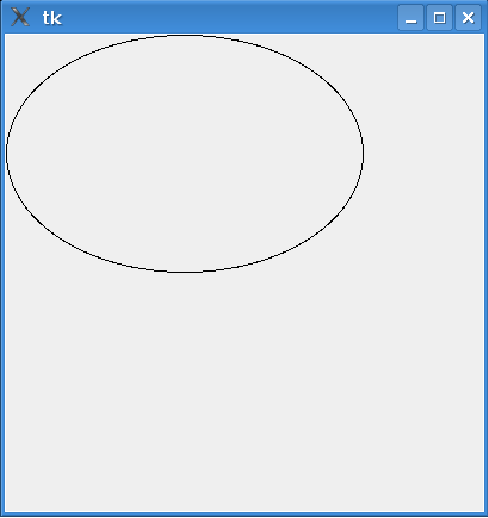
\includegraphics[width=80mm]{images/figure38}
%\end{center}
%\caption{The outline of an oval.}\label{fig38}
%\end{figure}
%% Diesel Bild (reine Ellipse) weggelassen, da kein erkennbarer Mehrwert zu figure39.

%\begin{figure}
%\begin{center}
%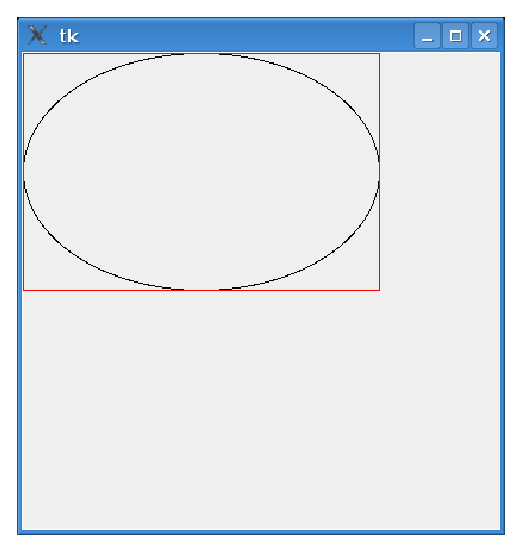
\includegraphics[width=80mm]{images/figure39}
%\end{center}
%\caption{The outline of an oval inside a rectangle.}\label{fig39}
%\end{figure}
\begin{figure}
\begin{center}
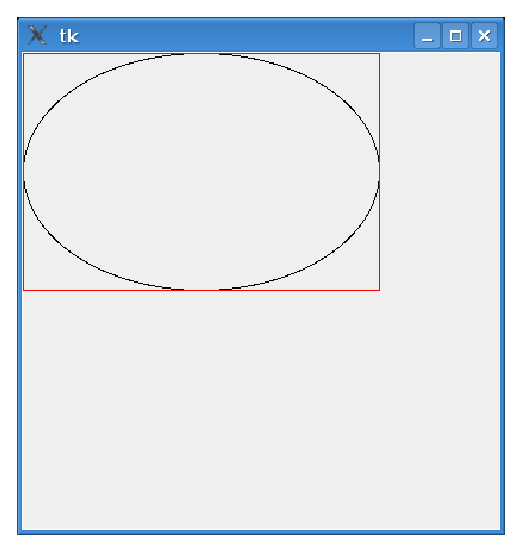
\includegraphics[width=80mm]{images/figure39}
\end{center}
\caption{Die Ellipse innerhalb des roten Rechtecks.}\label{fig39}
\end{figure}

\noindent
%To draw a circle, rather than an elliptical oval, the imaginary rectangle should be a square (which produces the circle in figure~\ref{fig40}):
Um einen Kreis anstatt einer Ellipse zu zeichnen, muss das imaginäre Rechteck quadratisch sein (siehe Abbildung~\ref{fig40}):

%\begin{Verbatim}[frame=single]
%>>> tk = Tk()
%>>> canvas = Canvas(tk, width=400,height=400)
%>>> canvas.pack()
%>>> canvas.create_oval(1, 1, 300, 300)
%\end{Verbatim}
\begin{Verbatim}[frame=single]
>>> tk = Tk()
>>> leinwand = Canvas(tk, width=400,height=400)
>>> leinwand.pack()
>>> leinwand.create_oval(1, 1, 300, 300)
\end{Verbatim}

%\begin{figure}
%\begin{center}
%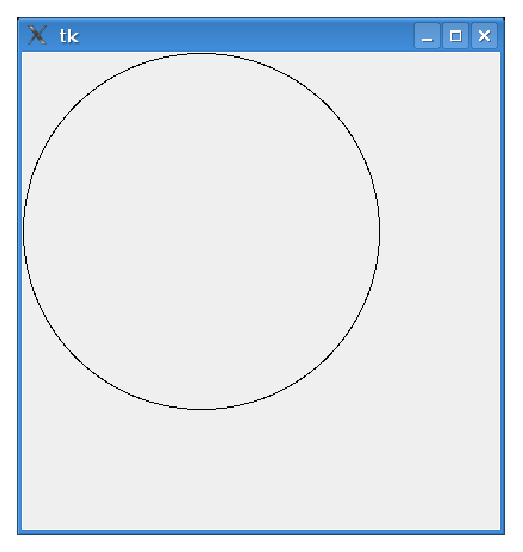
\includegraphics[width=80mm]{images/figure40}
%\end{center}
%\caption{A simple circle.}\label{fig40}
%\end{figure}
\begin{figure}
\begin{center}
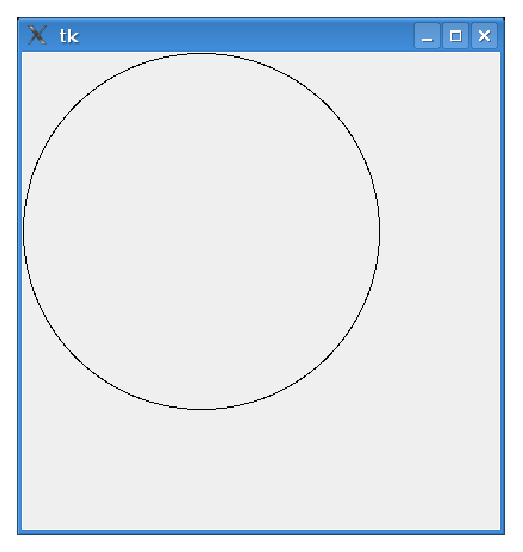
\includegraphics[width=80mm]{images/figure40}
\end{center}
\caption{Ein einfacher Kreis.}\label{fig40}
\end{figure}

%\section{Drawing Polygons}\index{modules!tkinter!create\_polygon}
\section{Polygone}\index{Module!tkinter!create\_polygon}

%A polygon is any shape with 3 or more sides. Triangles, squares, rectangles, pentagons, hexagons, and so on are all examples of polygons. As well as these more regular shapes, you can also create irregular shaped polygons. For example, to draw a triangle, you need to provide 3 sets of coordinates (that's a position across plus a position down) for each point of the triangle (creating the triangle in figure~\ref{fig41}):
Ein Polygon ist eine Form mit mehr als drei Seiten. Dreiecke, Vierecke, Fünfecke, Sechsecke und so weiter sind Beispiele dafür. Und die Formen können auch ganz ungleichmäßig sein. Für ein Dreieck musst du 3 Koordinatenpaare angeben (für jeden Eckpunkt). 

%\begin{Verbatim}[frame=single]
%>>> from tkinter import *
%>>> tk = Tk()
%>>> canvas = Canvas(tk, width=400,height=400)
%>>> canvas.pack()
%>>> canvas.create_polygon(10, 10, 100, 10, 100, 50, fill="", outline="black")
%\end{Verbatim}
\begin{Verbatim}[frame=single]
>>> from tkinter import *
>>> tk = Tk()
>>> leinwand = Canvas(tk, width=400,height=400)
>>> leinwand.pack()
>>> leinwand.create_polygon(10,10,100,10,100,50,fill="",outline="black")
\end{Verbatim}

Das Ergebnis siehst du in Abbildung~\ref{fig41}.

%\begin{figure}
%\begin{center}
%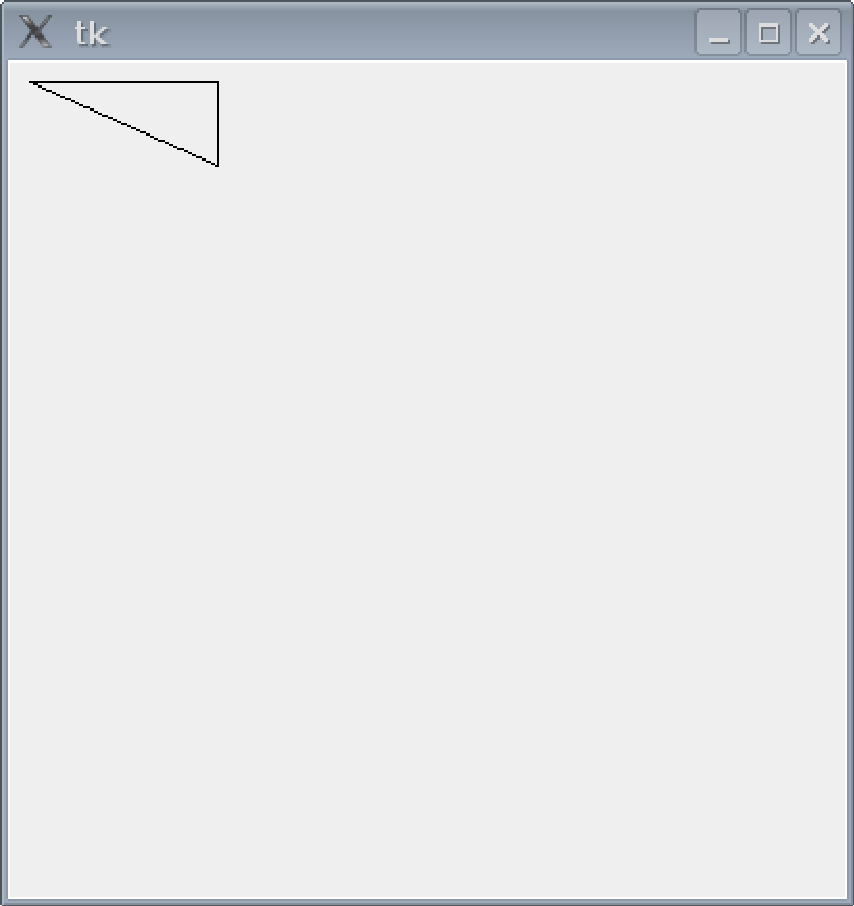
\includegraphics[width=80mm]{images/figure41}
%\end{center}
%\caption{A simple triangle.}\label{fig41}
%\end{figure}
\begin{figure}
\begin{center}
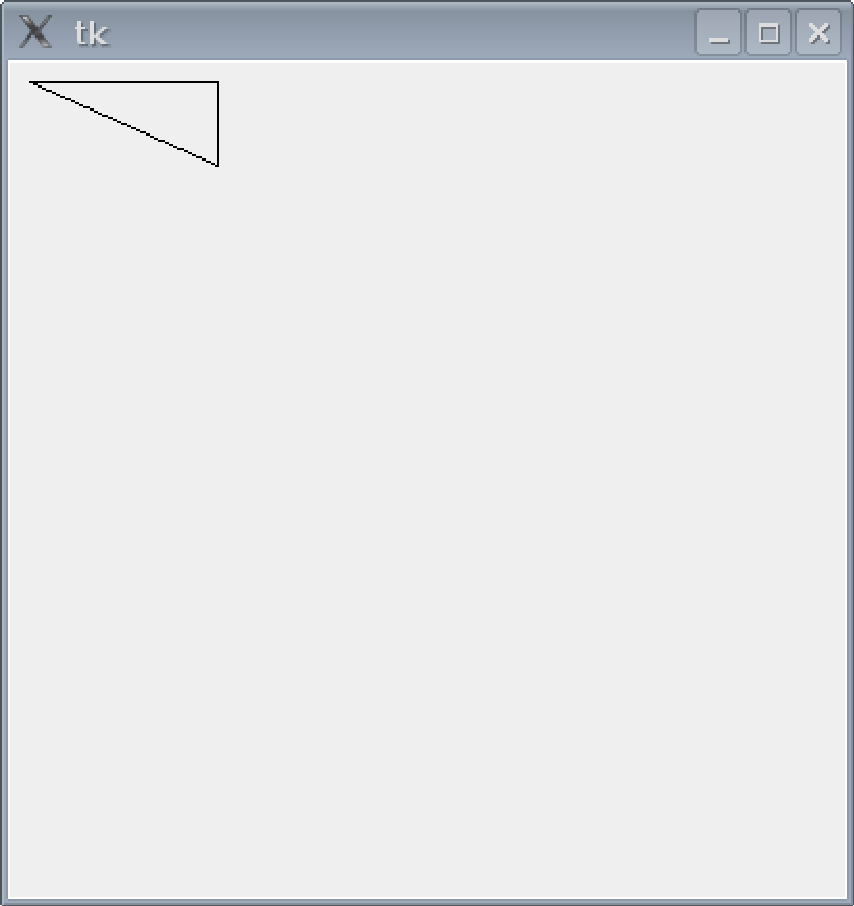
\includegraphics[width=80mm]{images/figure41}
\end{center}
\caption{Ein einfaches Dreieck.}\label{fig41}
\end{figure}

%We can add an irregular polygon using the following code. Figure~\ref{fig42} shows both the triangle and the oddly shaped polygon.
Zeichnen wir jetzt da noch ein unregelmäßiges Vieleck mit dem folgenden Code dazu.

%\begin{Verbatim}[frame=single]
%>>> canvas.create_polygon(200, 10, 240, 30, 120, 100, 140, 120, fill="", outline="black")
%\end{Verbatim}
\begin{Verbatim}[frame=single]
>>> leinwand.create_polygon(200,10,240,30,120,100,140,120,fill="",outline="black")
\end{Verbatim}

Dreieck und Vieleck siehst du in Abbildung~\ref{fig42}.

%\begin{figure}
%\begin{center}
%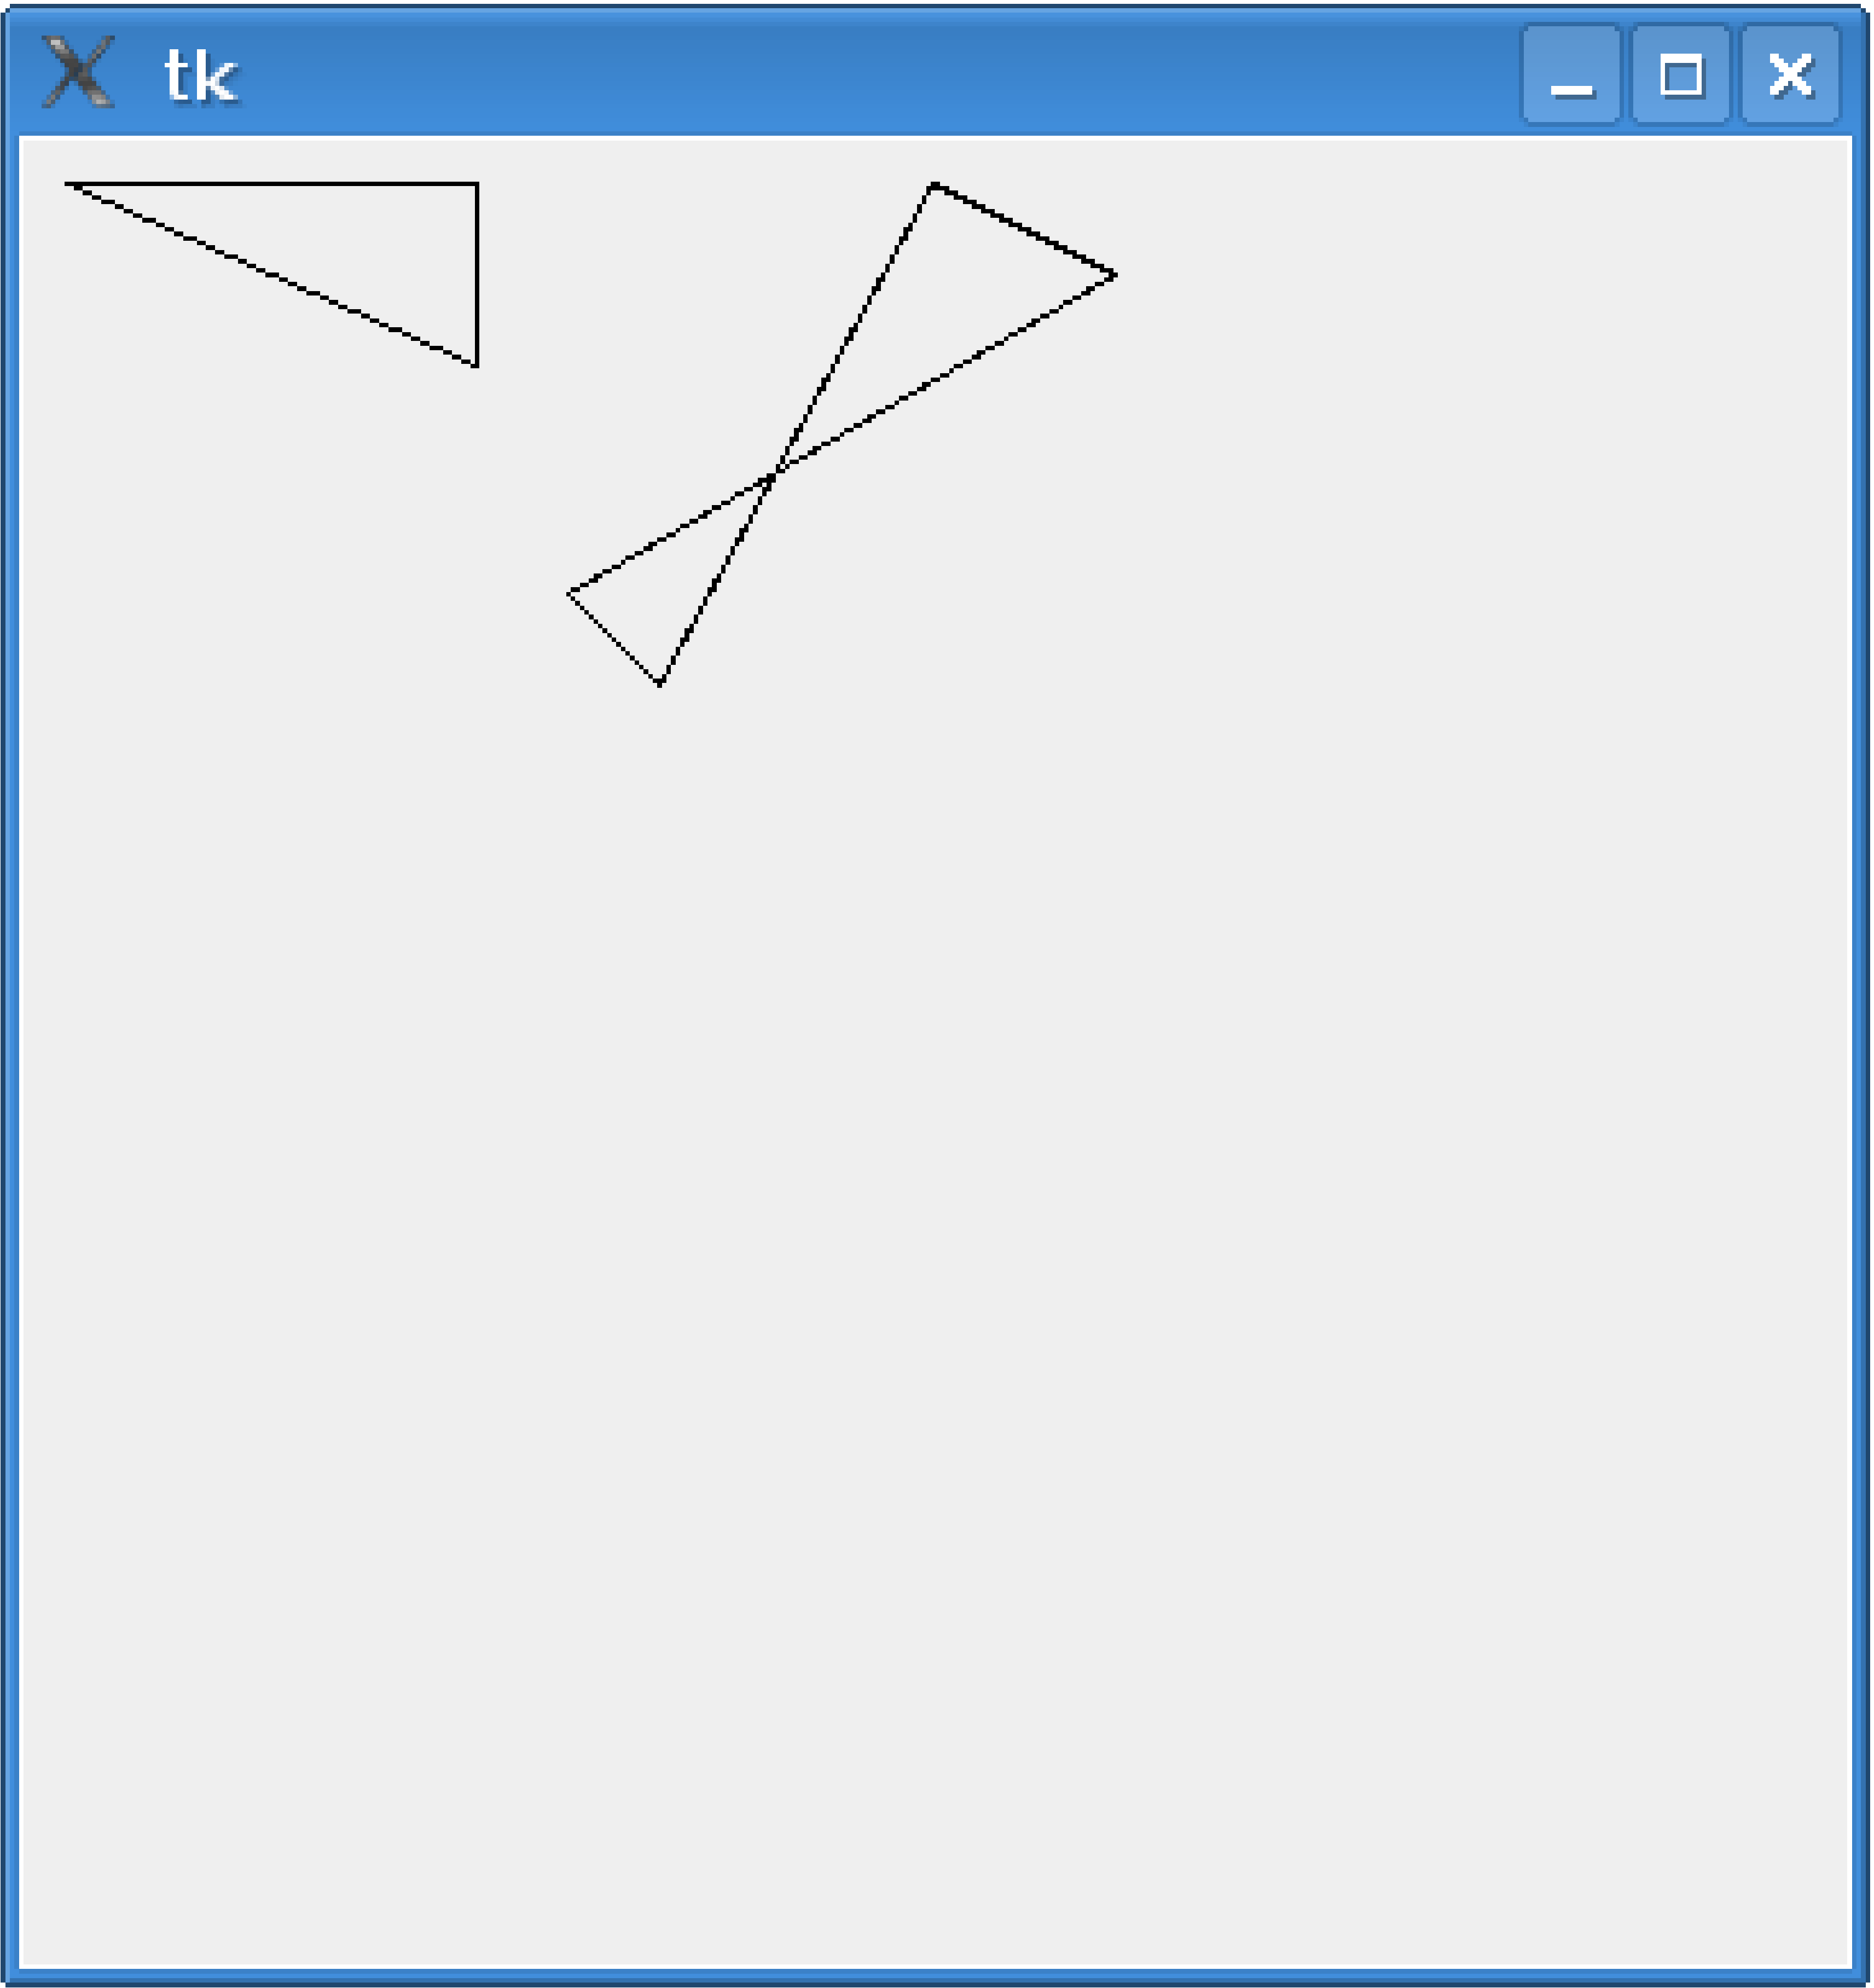
\includegraphics[width=80mm]{images/figure42}
%\end{center}
%\caption{A simple triangle.}\label{fig42}
%\end{figure}
\begin{figure}
\begin{center}
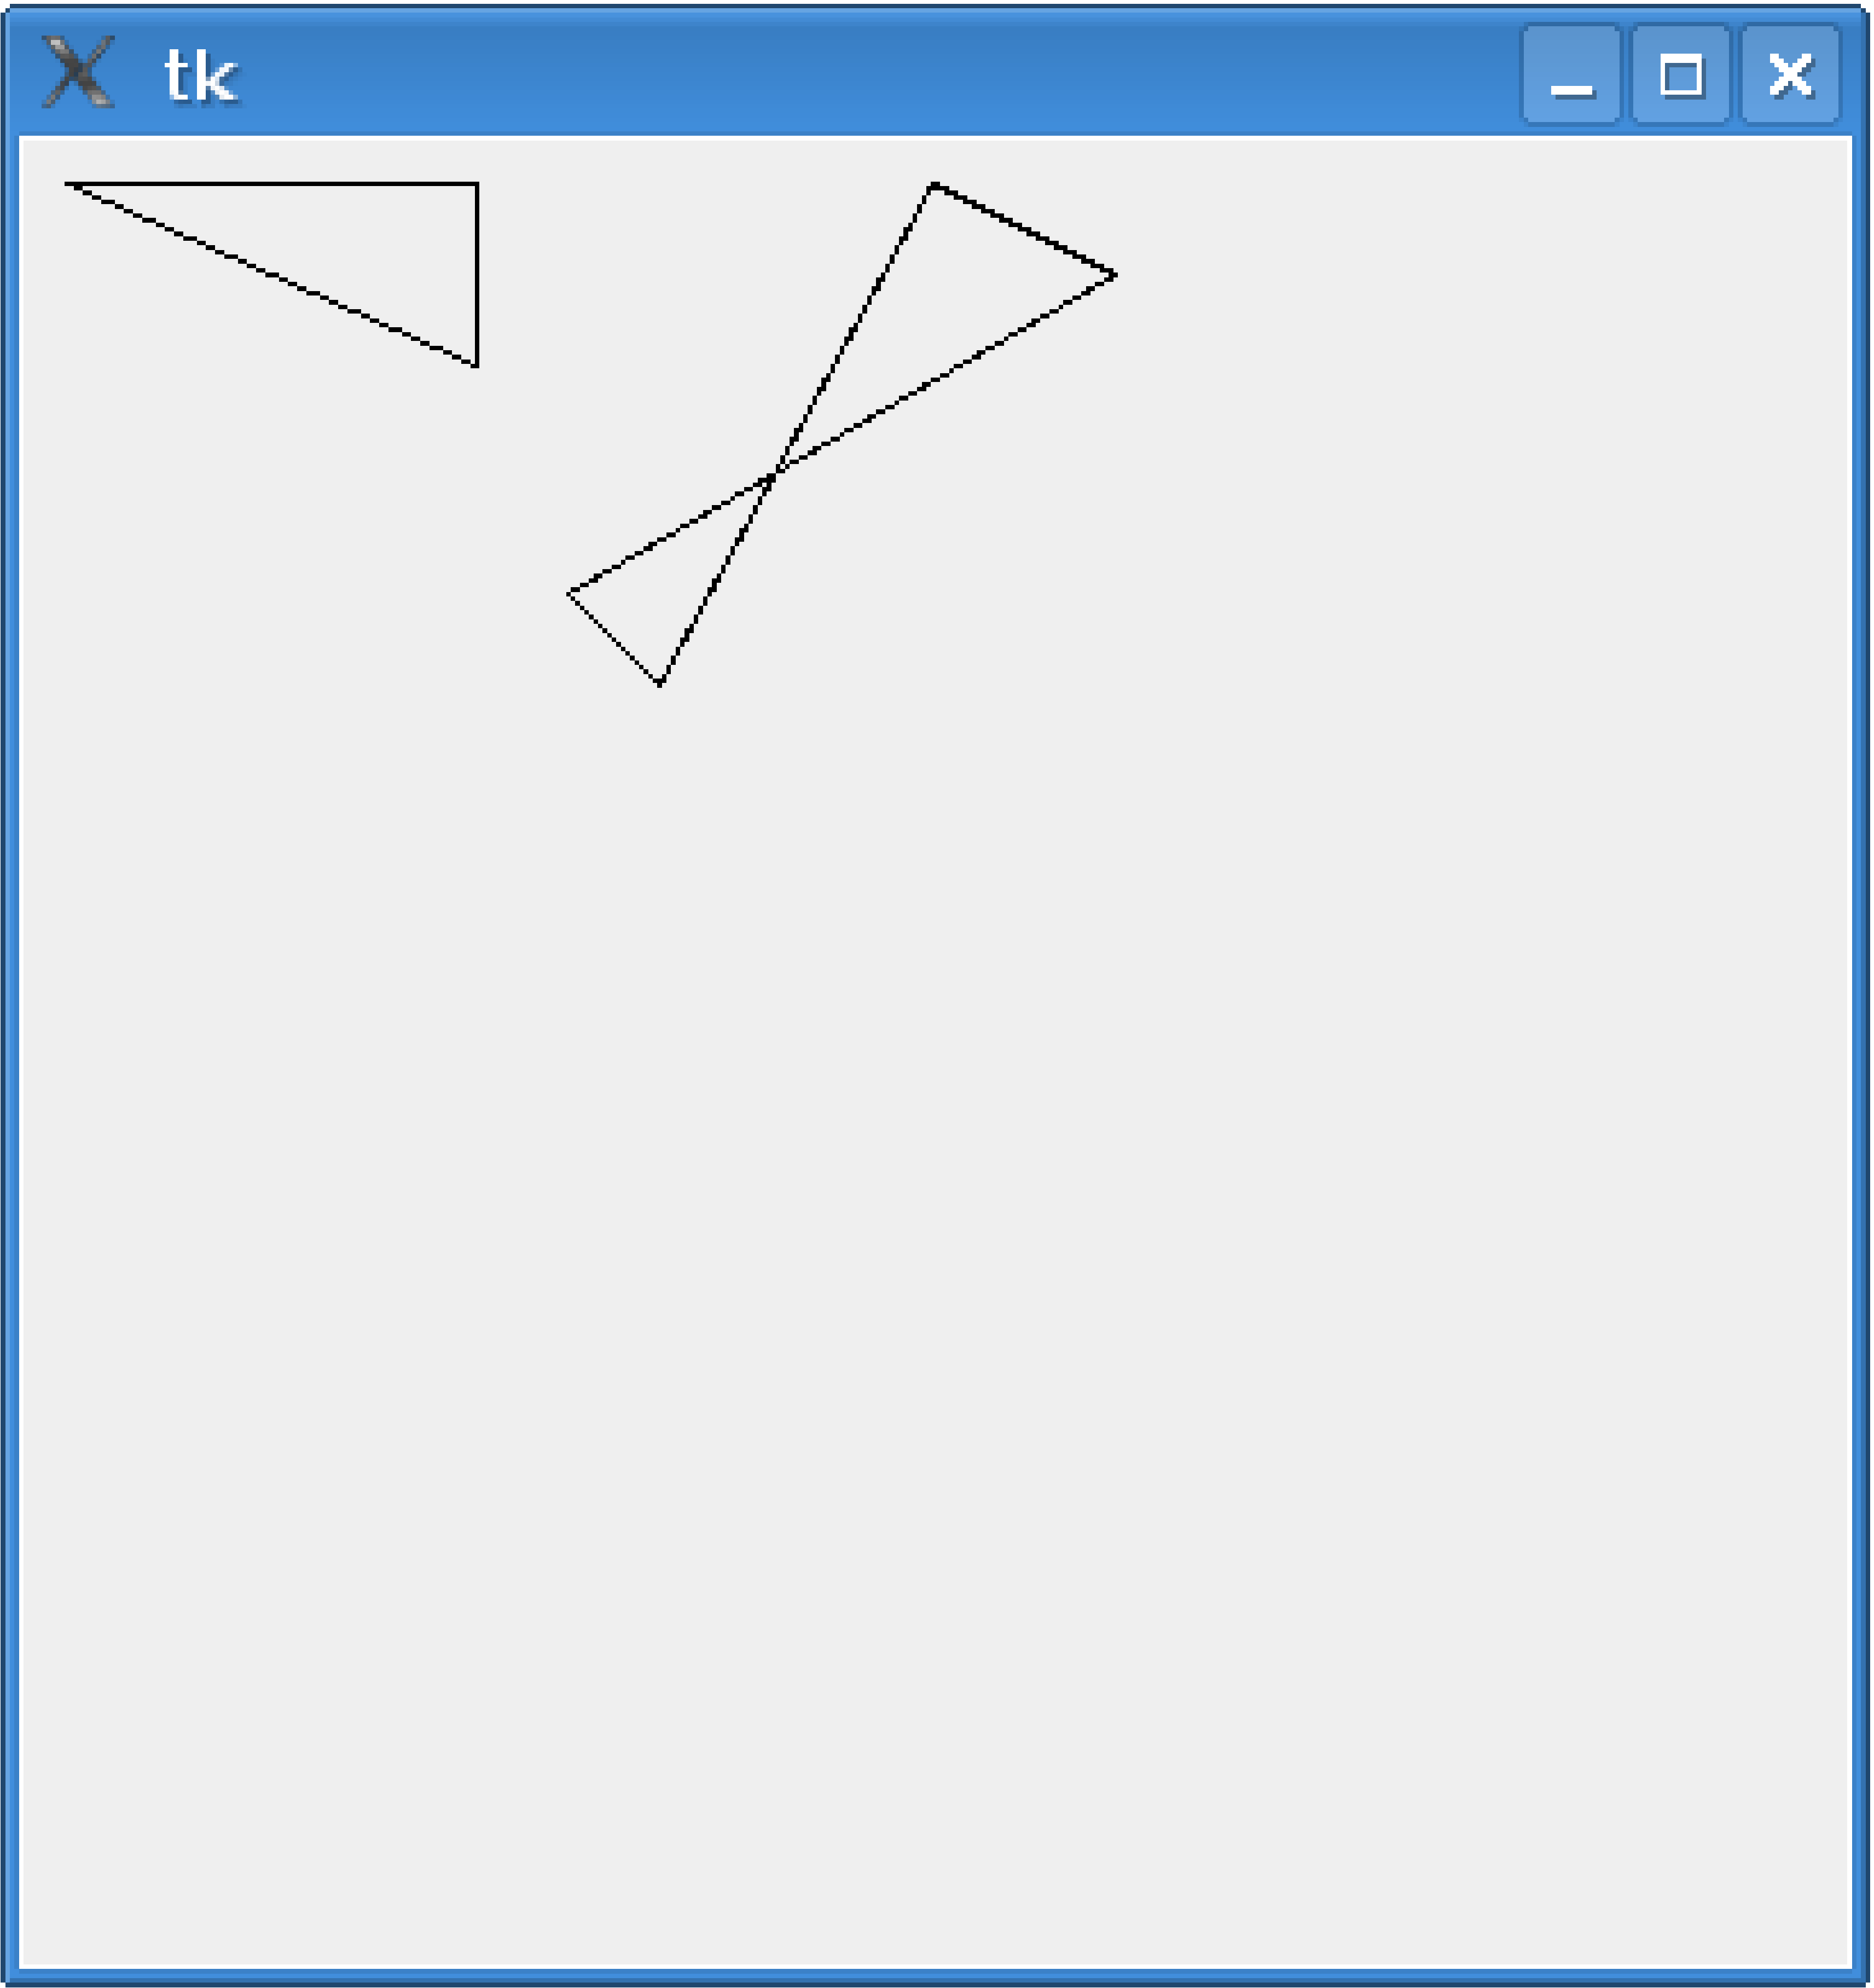
\includegraphics[width=80mm]{images/figure42}
\end{center}
\caption{Das Dreieck und das unregelmäßige Vieleck.}\label{fig42}
\end{figure}

%\section{Drawing Images}
\section{Zeichne Bilder}
%You can draw an image on a canvas using \code{tkinter} by first loading the image, then using the \code{create\_image}\index{modules!tkinter!create\_image} function on the canvas object. This sounds a bit illogical, but it works as follows:
Du kannst auch Bilder auf die Leinwand laden. Zuerst lädst du das Bild, dann benützt du die Funktion \code{create\_image}\index{Module!tkinter!create\_image} und es erscheint auf der Leinwand. Probiere es aus:

%\begin{Verbatim}[frame=single]
%1. >>> from tkinter import *
%2. >>> tk = Tk()
%3. >>> canvas = Canvas(tk, width=400, height=400)
%4. >>> canvas.pack()
%5. >>> myimage = PhotoImage(file='test.gif')
%6. >>> canvas.create_image(0, 0, image=myimage, anchor=NW)
%\end{Verbatim}
\begin{Verbatim}[frame=single]
1. >>> from tkinter import *
2. >>> tk = Tk()
3. >>> leinwand = Canvas(tk, width=400, height=400)
4. >>> leinwand.pack()
5. >>> mein_bild = PhotoImage(file='test.gif')
6. >>> canvas.create_image(0, 0, image=mein_bild, anchor=NW)
\end{Verbatim}

%In lines 1 to 4 we set up the canvas the same as we have in previous examples. In line 5, the image is loaded into the variable \code{myimage}. It's important that the image you want to load is in a directory that's accessible to Python. This is usually the directory that the Python console is running from. You can find out the name of this directory by importing the \code{os}\index{modules!os} module and using the \code{getcwd()} function:
In den ersten 4 Zeilen generieren wir wieder die Leinwand wie in den vorigen Beispielen. In der fünften Zeile laden wir dann das Bild in die Variable \code{mein\_bild}. Das Bild muss in einem Ordner liegen, auf den Python zugreifen kann. Normalerweise ist dies das Verzeichnis in dem die Python-Konsole gestartet wurde. Wo genau dieses Verzeichnis ist, kannst du leicht herausfinden. Importiere das \code{os}\index{Module!os}-Modul und verwende die \code{getcwd()}-Funktion: 

%\begin{Verbatim}[frame=single]
%>>> import os
%>>> print(os.getcwd())
%\end{Verbatim}
\begin{Verbatim}[frame=single]
>>> import os
>>> print(os.getcwd())
\end{Verbatim}

\begin{WINDOWS}
%This will probably print out something like `c:\\Python30'.
Unter Windows wirst du vermutlich etwas wie `c:\\Python30' bekommen.
\end{WINDOWS}

\begin{MAC}
%This will probably print out something like `/Users/yourname'\texorpdfstring{$\ldots$}{...}, so if your name is Jane Matthews, \code{getcwd()} might return `/Users/janematthews'.
Wenn du einen Mac verwendest wirst du etwas wie `/Users/dein\_name' \texorpdfstring{$\ldots$}{...} bekommen. 
\end{MAC}

\begin{LINUX}
%This will probably print out something like `/home/yourname'\texorpdfstring{$\ldots$}{...}, so if your name is Jane Matthews, \code{getcwd()} might return `/home/jane' or `/home/janematthews', depending upon how your computer has been setup.
Mit Linux wirst du etwas wie `/home/dein\_name' \texorpdfstring{$\ldots$}{...} zurückbekommen. Wenn du also Jana Thaler heißt, könnte die Ausgabe von \code{getcwd()} etwa `/home/jana' oder `/home/janathaler' ausgeben, je nachdem, wie der Computer installiert wurde.
\end{LINUX}

%Copy your image into that directory and then load it using the PhotoImage function (same as line 5). You then use the \code{create\_image} function on the canvas to display your image (line 6). If you've done all this correctly, you'll see something like figure~\ref{fig43}.
Kopiere nun das Bild ins Verzeichnis und lade es mit der PhotoImage-Funktion (siehe Zeile 5). Dann benützt du die \code{create\_image}-Funktion um das Bild auf der Leinwand zu befestigen. Das Ergebnis könnte wie Abbildung~\ref{fig43} aussehen.

%\begin{figure}
%\begin{center}
%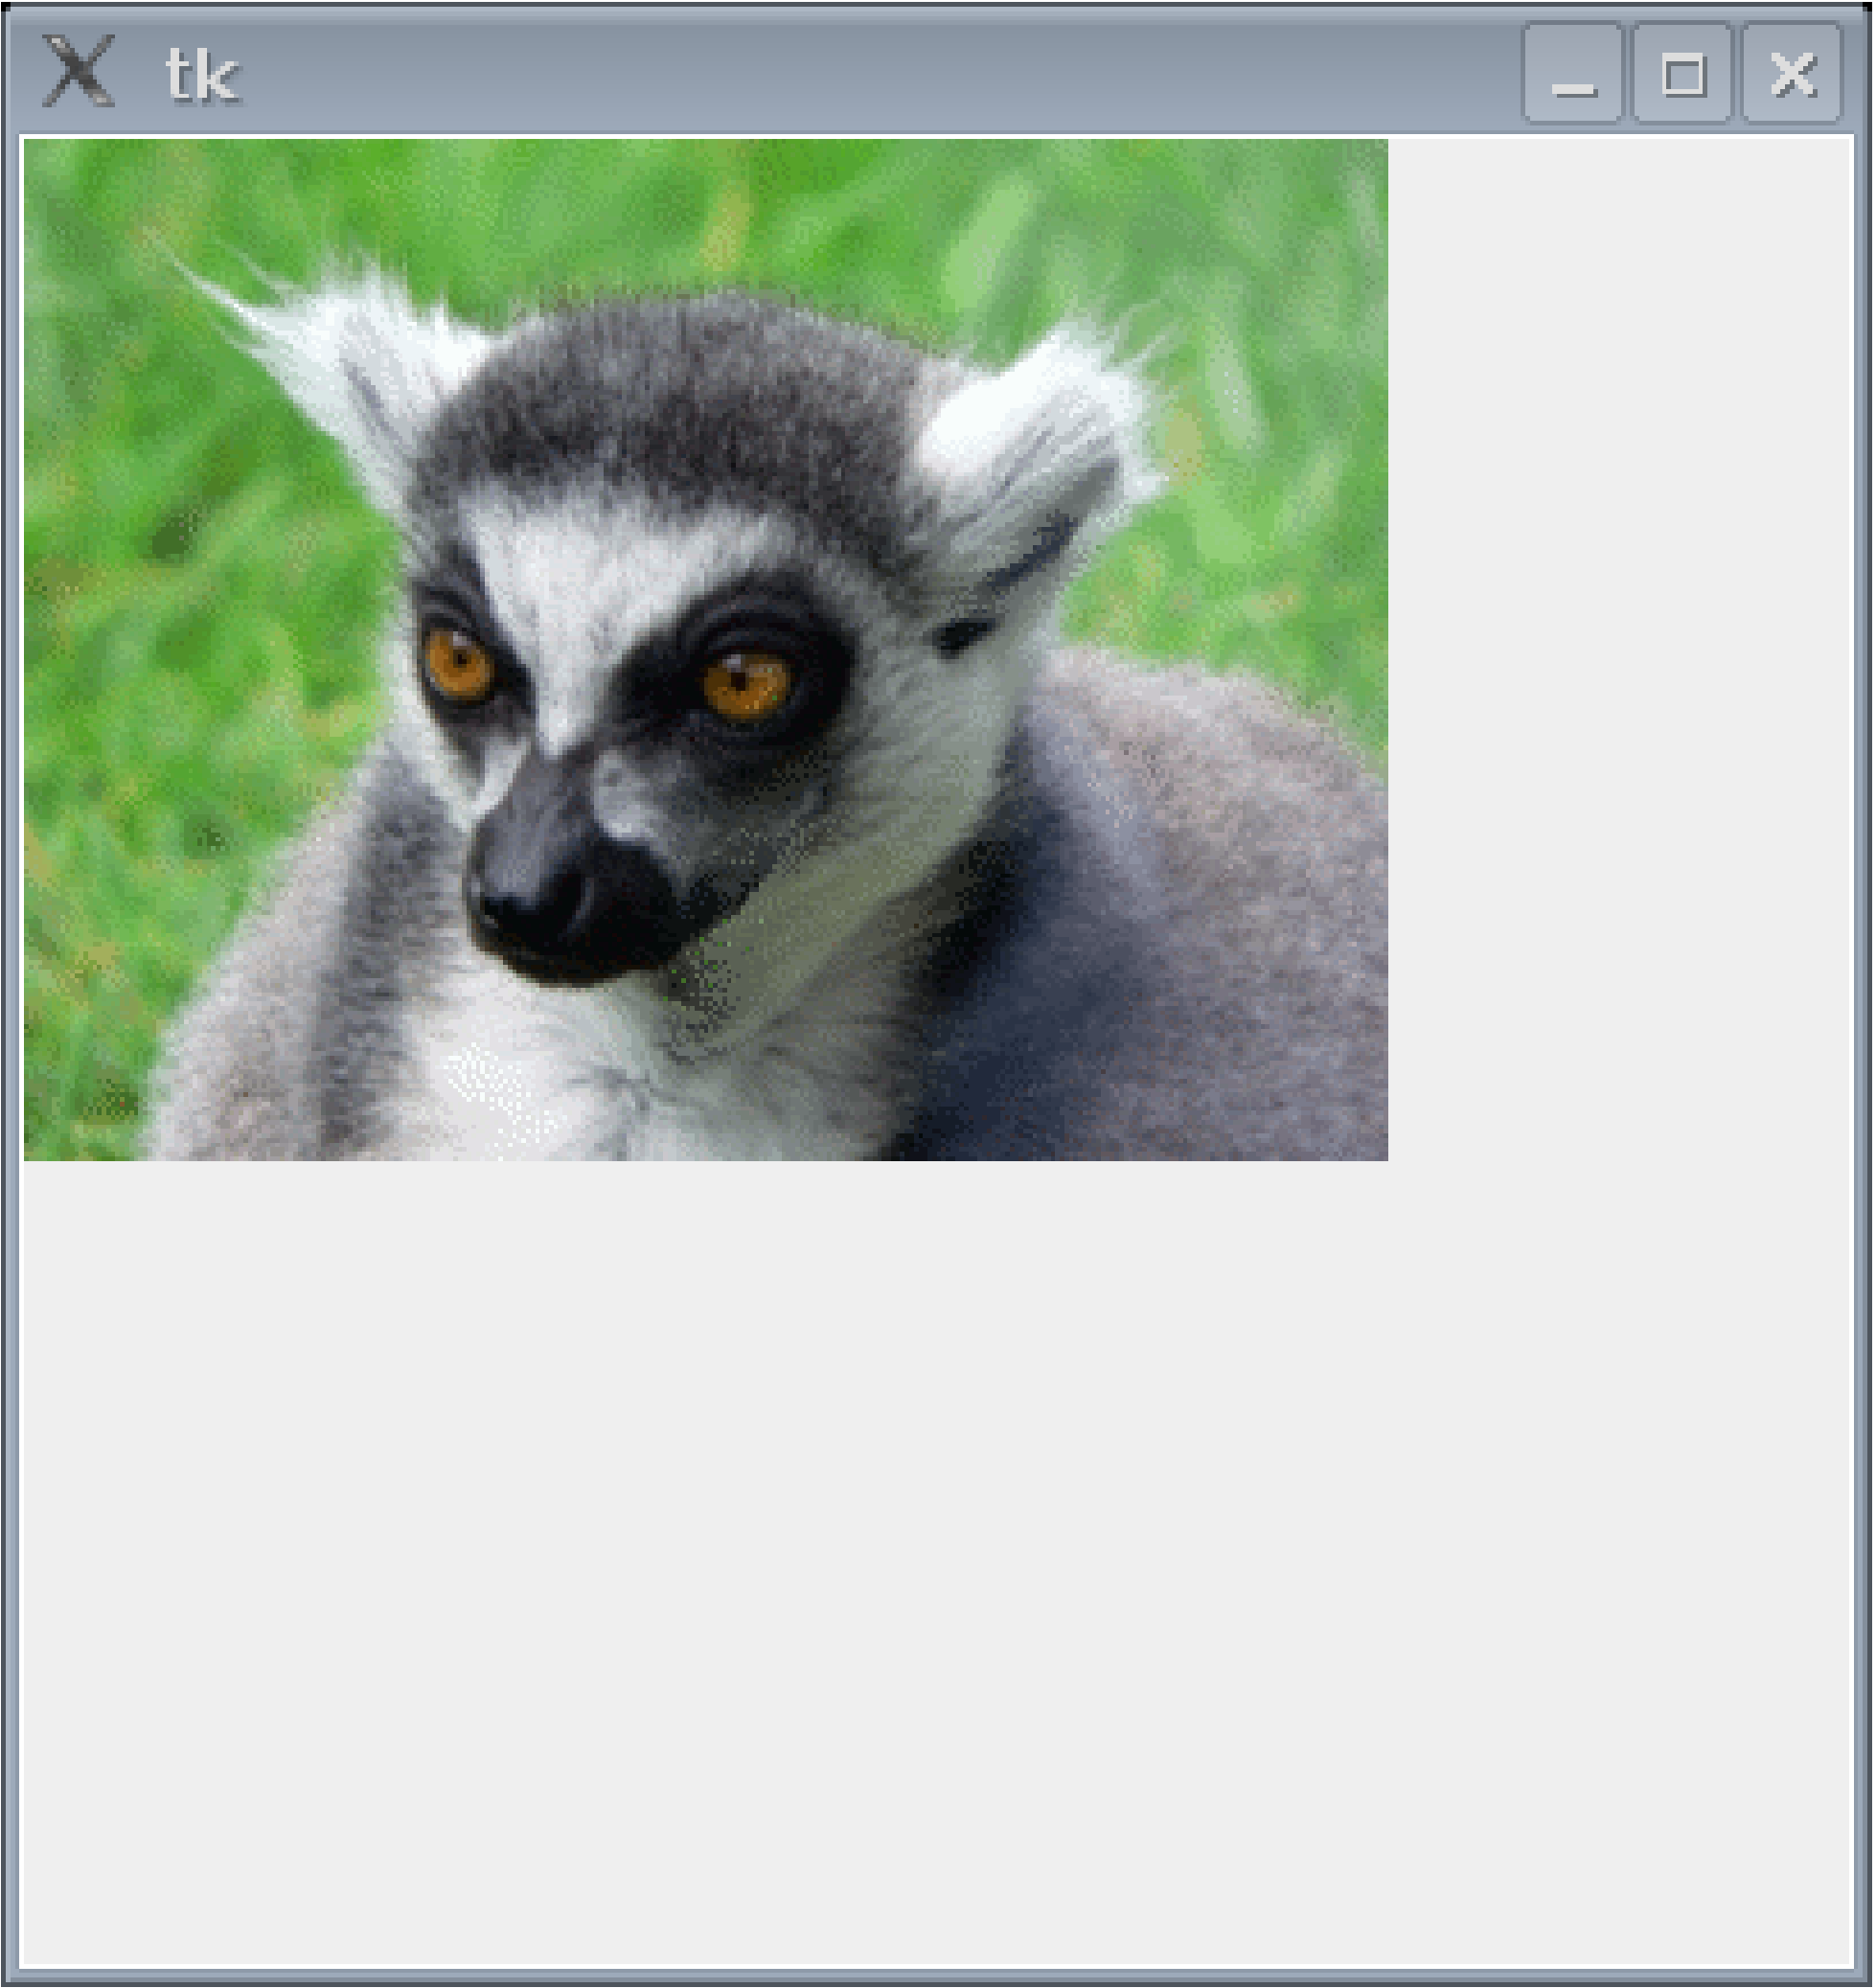
\includegraphics[width=80mm]{images/figure43}
%\end{center}
%\caption{A photo image.}\label{fig43}
%\end{figure}
\begin{figure}
\begin{center}
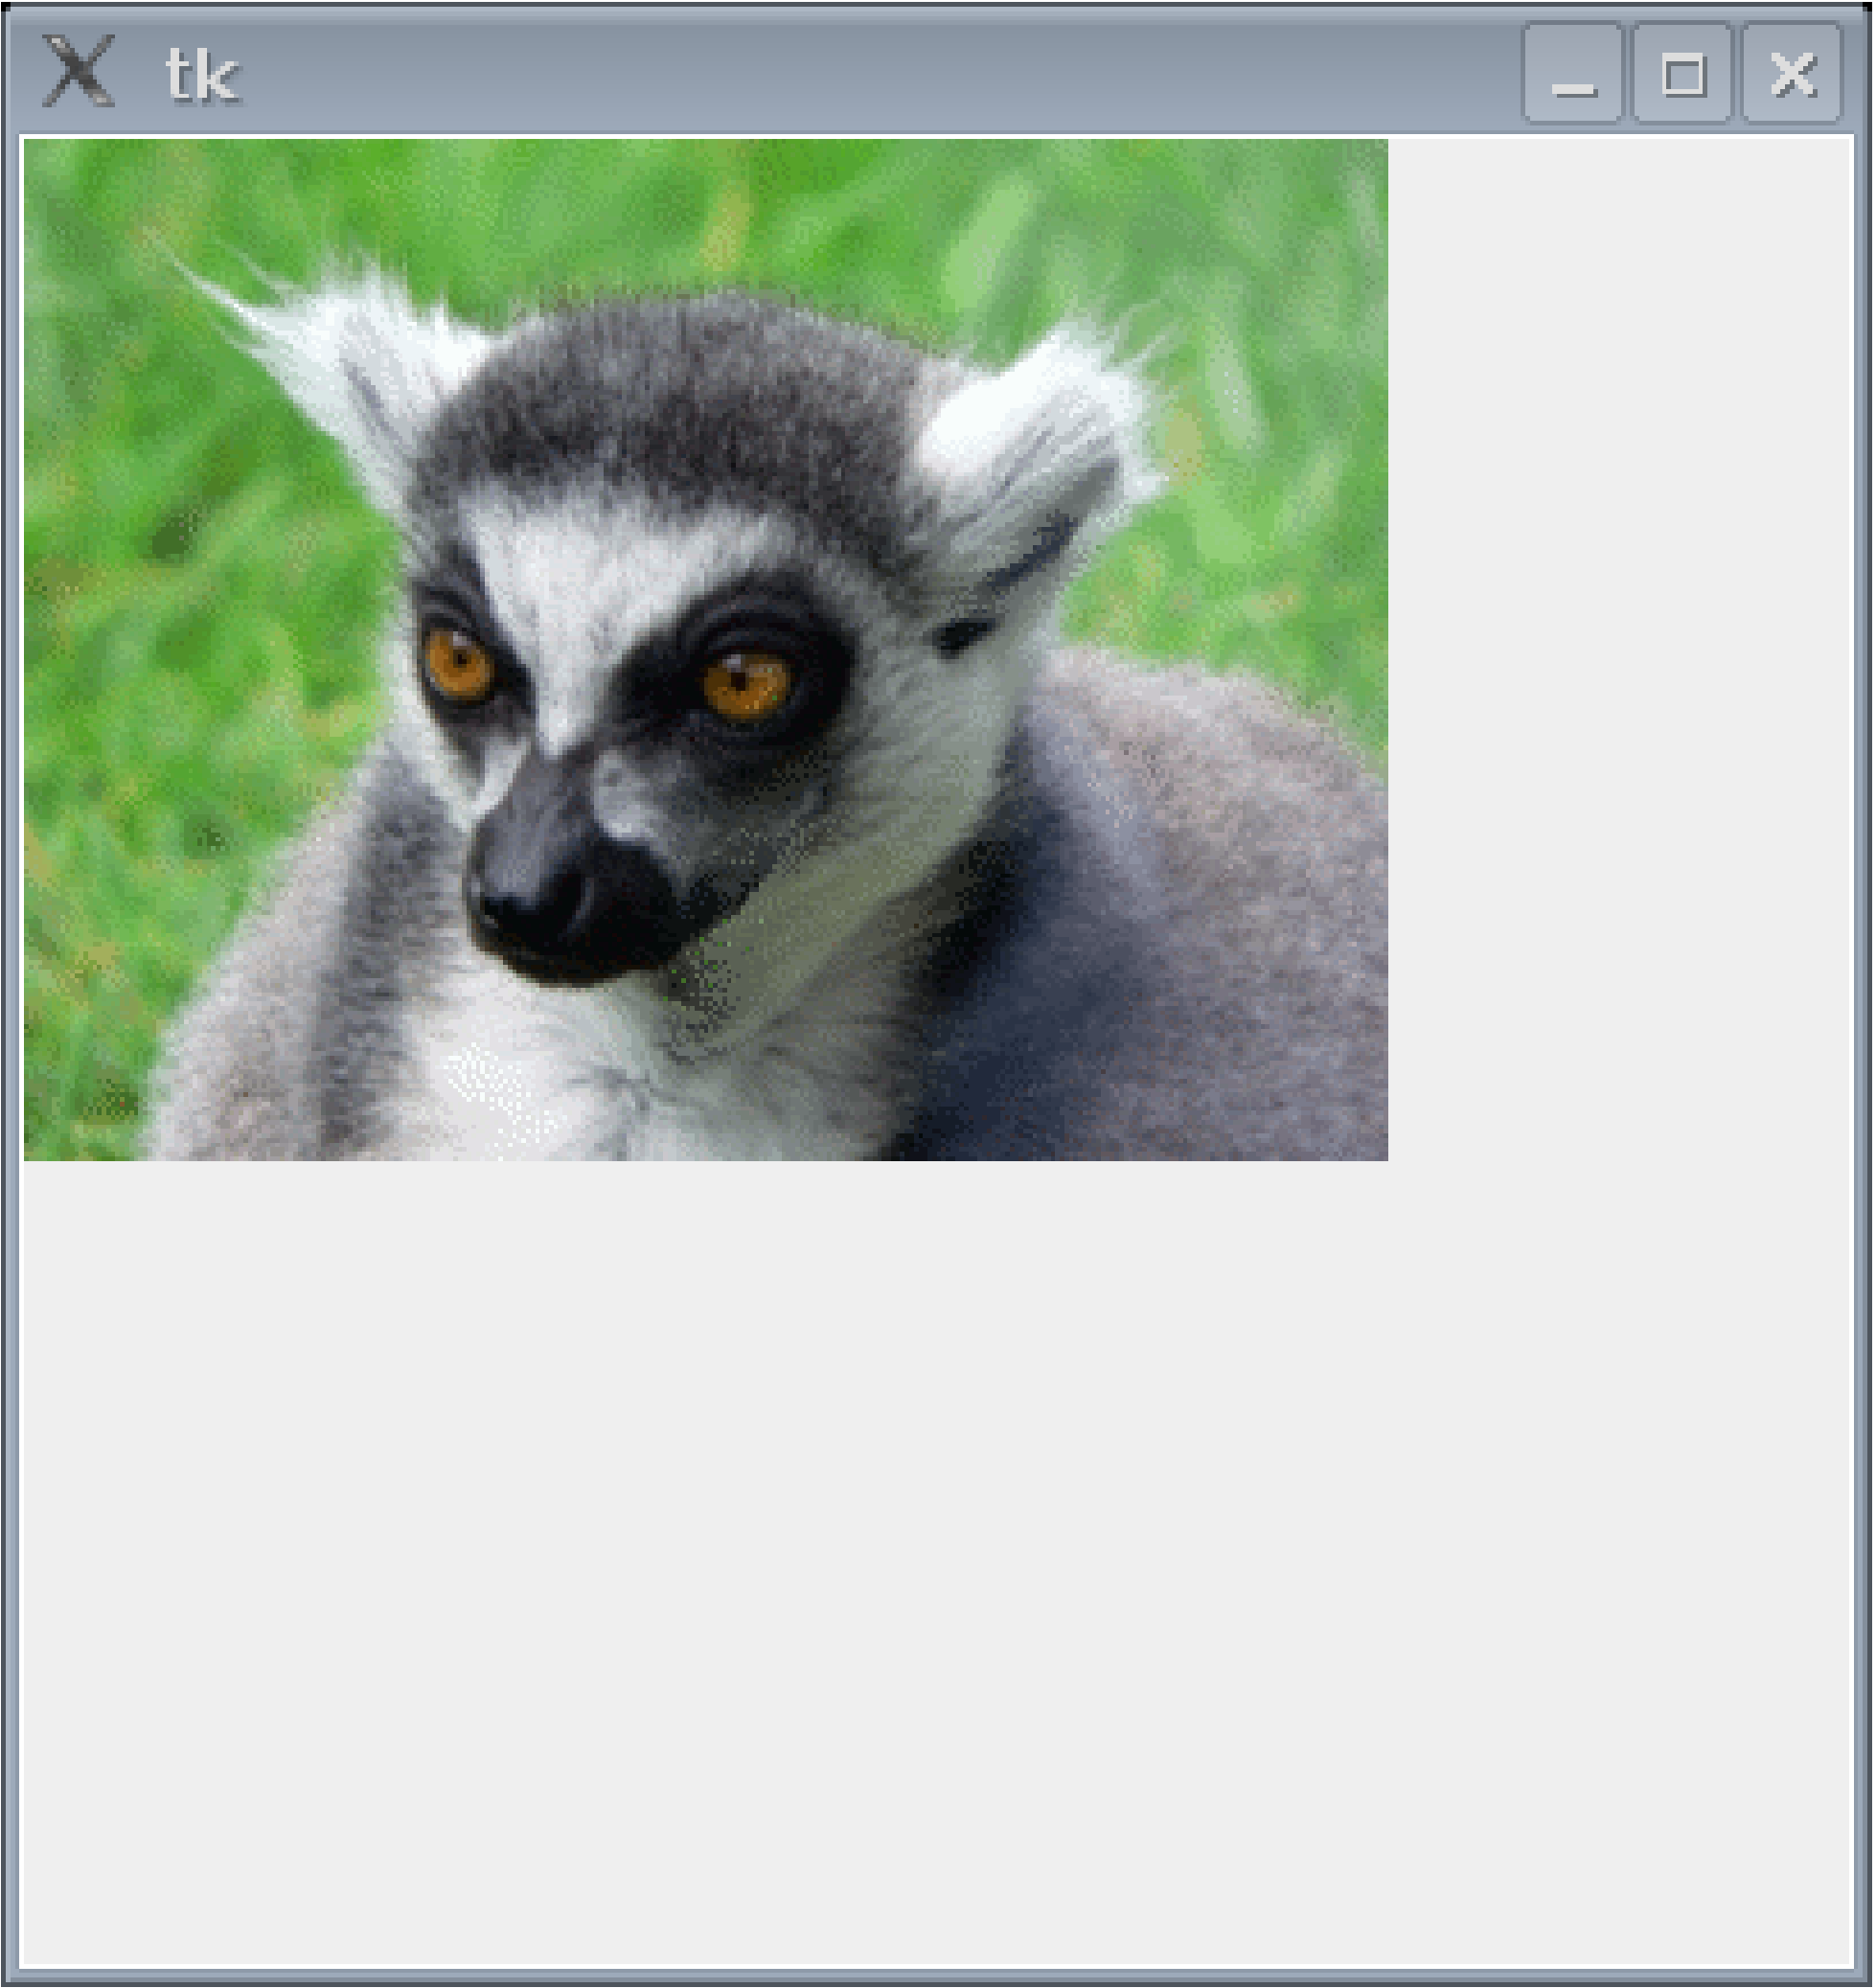
\includegraphics[width=80mm]{images/figure43}
\end{center}
\caption{Ein Photo auf der Leinwand.}\label{fig43}
\end{figure}

%PhotoImage can load image files with the extensions .gif, .ppm and .pgm. If you want to load other types of images (there are lots of different ways you can create image files---for example, digital cameras usually store images with the extension .jpg), then you'll need to use an extension which adds that capability to Python. The Python Imaging Library (PIL)\footnote{The Python Imaging Library can be found at \href{http://www.pythonware.com/products/pil/index.htm}{http://www.pythonware.com/products/pil/index.htm}} adds the ability to load all kinds of images, as well as do things like expand and shrink, change image colours, reverse images and so on. However, installing and using the Python Imaging Library, is a bit beyond the scope of this book.
Mit PhotoImage kannst du Dateien mit den Endungen .gif, .ppm und .pgm laden. Wenn du andere Bildformate laden willst (zum Beispiel speichern Digitalkameras Bilder meistens als .jpg), musst du zuerst eine Python Erweiterung laden. Die Python-Bilder-Bibliothek \footnote{Du findest die Python Bibliothek für Bilder unter \href{http://www.pythonware.com/products/pil/index.htm}{http://www.pythonware.com/products/pil/index.htm}} (Python Imaging Library auch PIL genannt) wäre ein Beispiel dafür.


%\section{Basic Animation}\index{modules!tkinter!basic animation}
\section{Einfache Animationen}\index{Module!tkinter!Einfache Animationen}

%So far, we've seen how to do static drawing---that's pictures that don't move. What about animation? Animation is not necessarily \code{Tk}'s strong suit, but you can do the basics. For example, we can create a filled triangle and then make it move across the screen using the following code:
Bis jetzt haben wir immer statische Bilder---das sind Bilder, die sich nicht bewegen, gezeichnet. Was ist mit Animationen? \code{Tk} ist zwar nicht direkt darauf ausgelegt, aber für einfache kleine Sachen reicht es schon. Zum Beispiel können wir ein Dreieck füllen und dann über den Bildschirm wandern lassen:

%\begin{Verbatim}[frame=single]
%1.  >>> import time
%2.  >>> from tkinter import *
%3.  >>> tk = Tk()
%4.  >>> canvas = Canvas(tk, width=400, height=400)
%5.  >>> canvas.pack()
%6.  >>> canvas.create_polygon(10, 10, 10, 60, 50, 35)
%7.  1
%8.  >>> for x in range(0, 60):
%9.  ...     canvas.move(1, 5, 0)
%10. ...     tk.update()
%11. ...     time.sleep(0.05)
%\end{Verbatim}
\begin{Verbatim}[frame=single]
1.  >>> import time
2.  >>> from tkinter import *
3.  >>> tk = Tk()
4.  >>> leinwand = Canvas(tk, width=400, height=400)
5.  >>> leinwand.pack()
6.  >>> leinwand.create_polygon(10, 10, 10, 60, 50, 35)
7.  1
8.  >>> for x in range(0, 40):
9.  ...     leinwand.move(1, 5, 0)
10. ...     tk.update()
11. ...     time.sleep(0.05)
\end{Verbatim}

%The moment you press the Enter key after typing the last line, the triangle will start moving across the screen (you can see it half-way across in figure~\ref{fig44}).
Wenn du nun nach dem letzten Befehl Enter drückst, wird sich das Dreieck über den Bildschirm bewegen (und dann nach 40 x 5 = 200 Pixeln etwa in der Mitte stehenbleiben wie in Abbildung~\ref{fig44}).

%\begin{figure}
%\begin{center}
%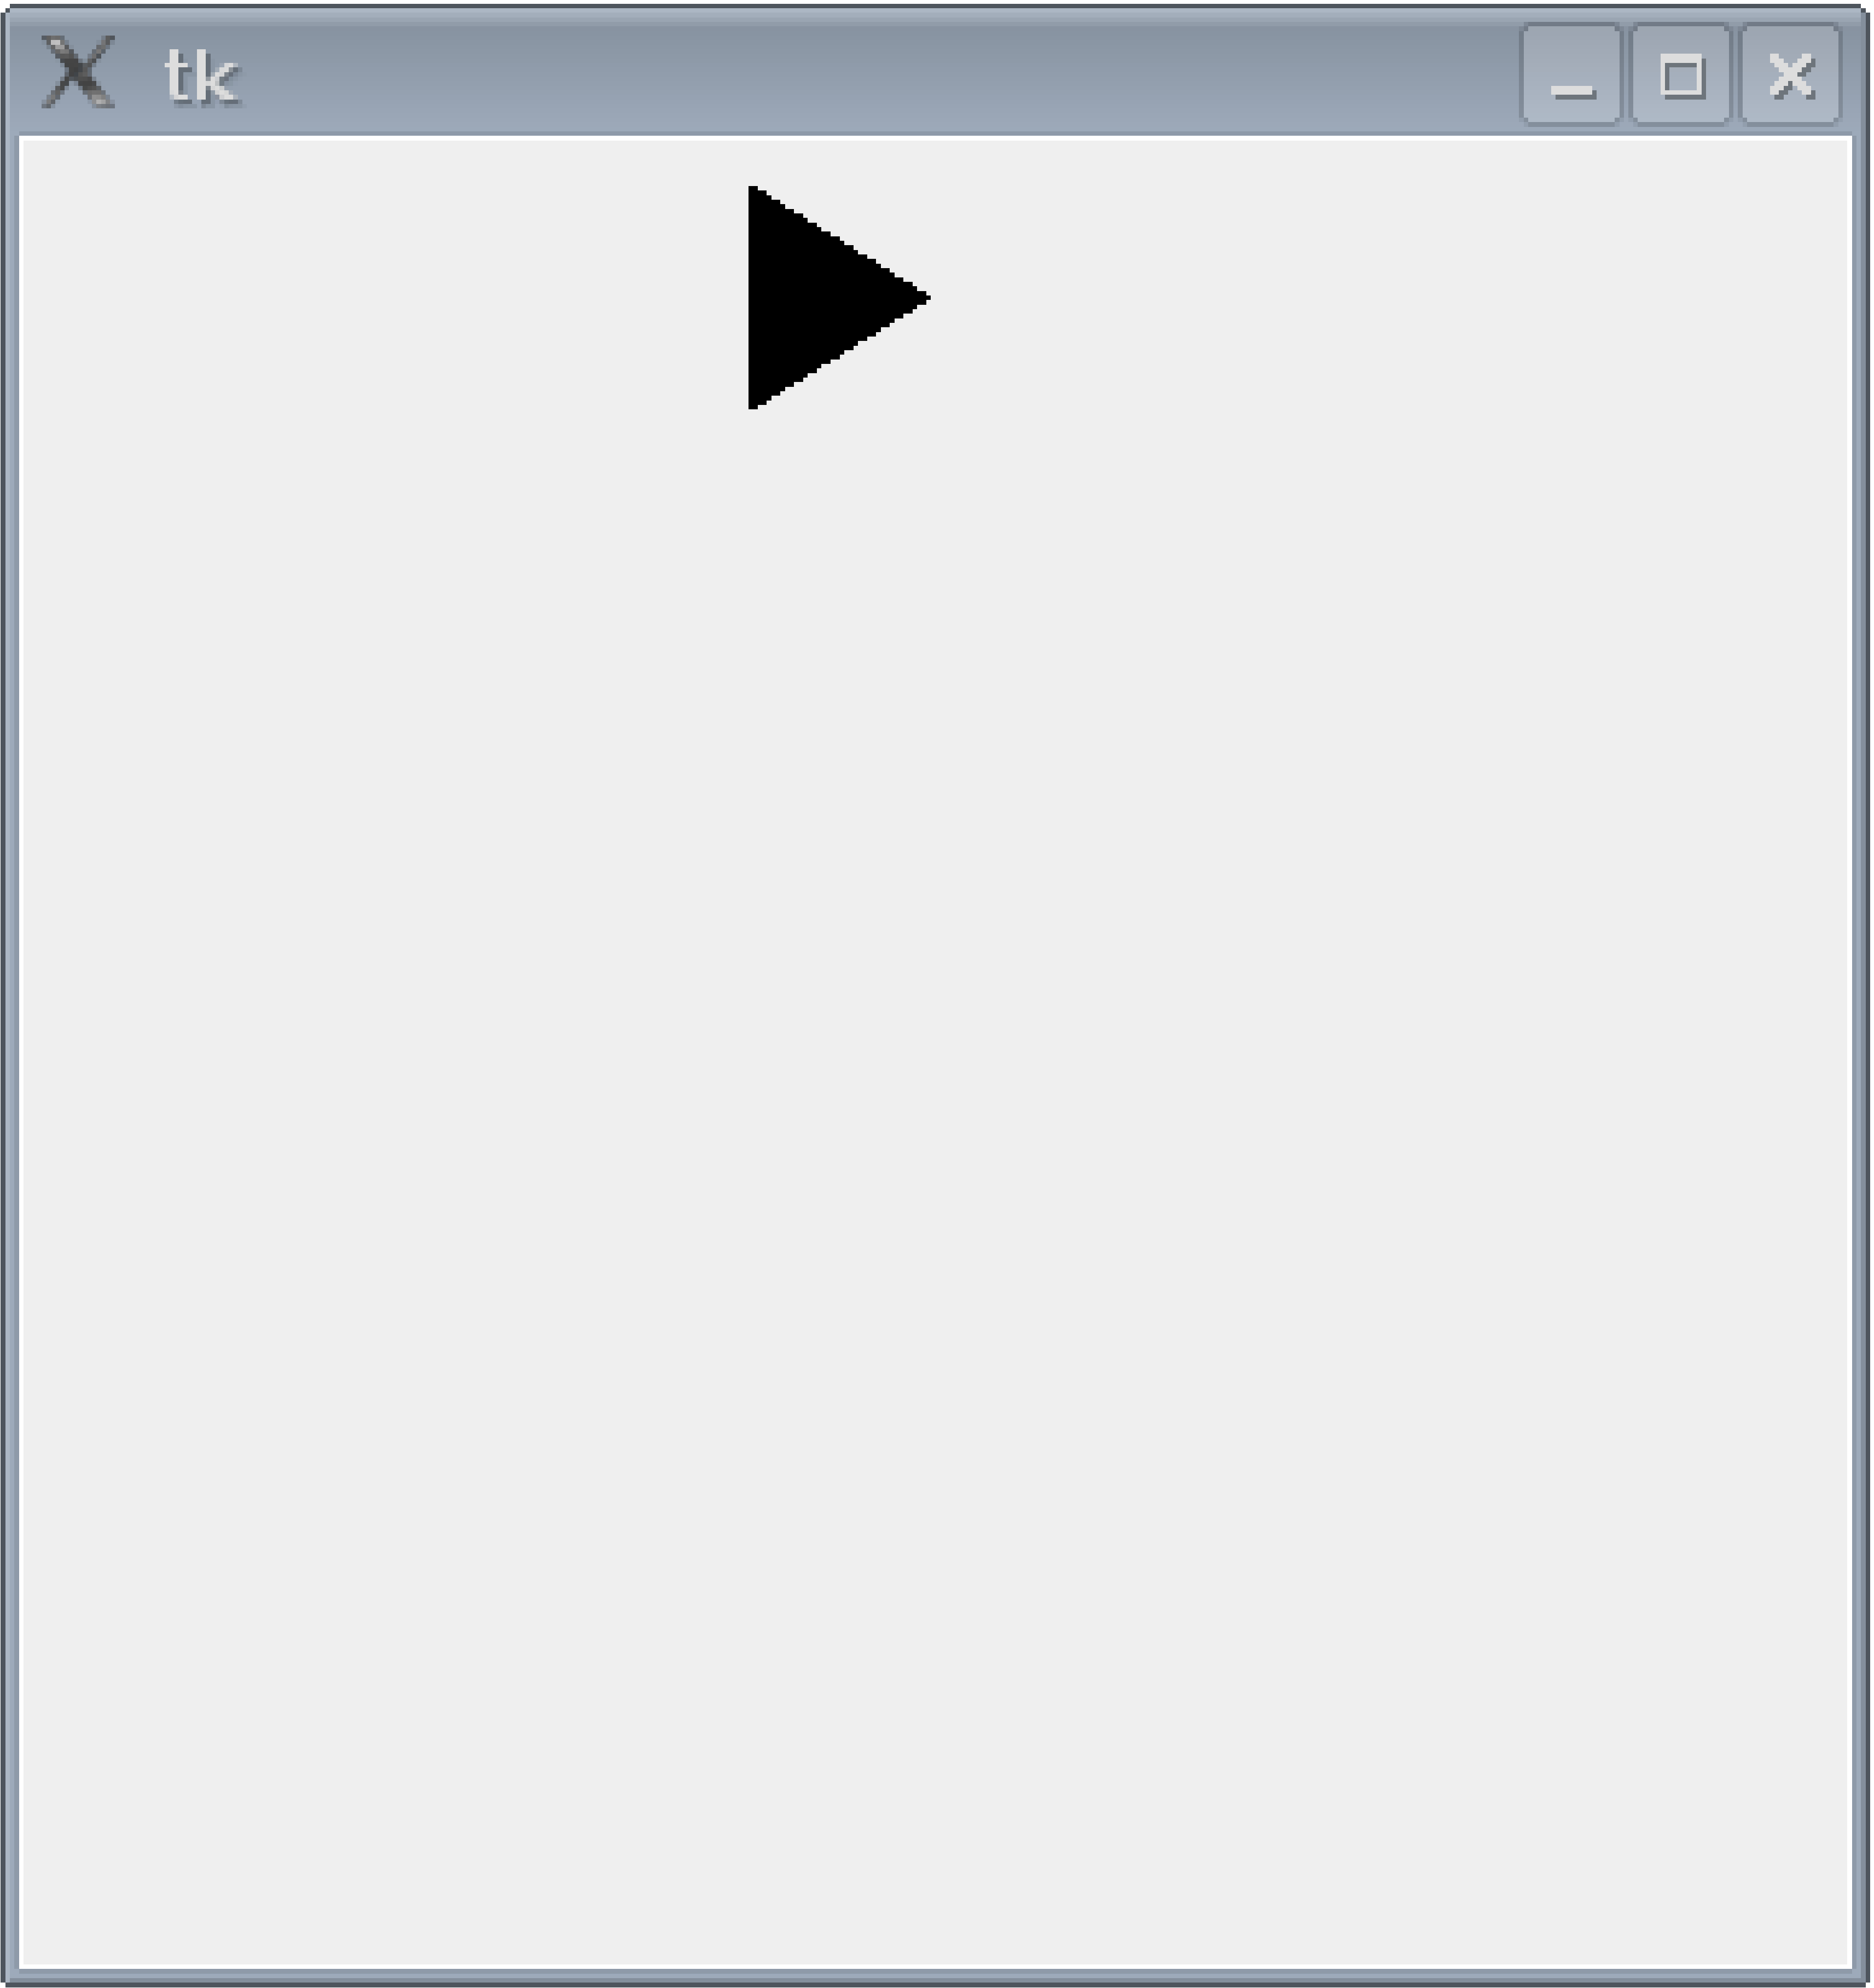
\includegraphics[width=80mm]{images/figure44}
%\end{center}
%\caption{The triangle moving across the screen.}\label{fig44}
%\end{figure}
\begin{figure}
\begin{center}
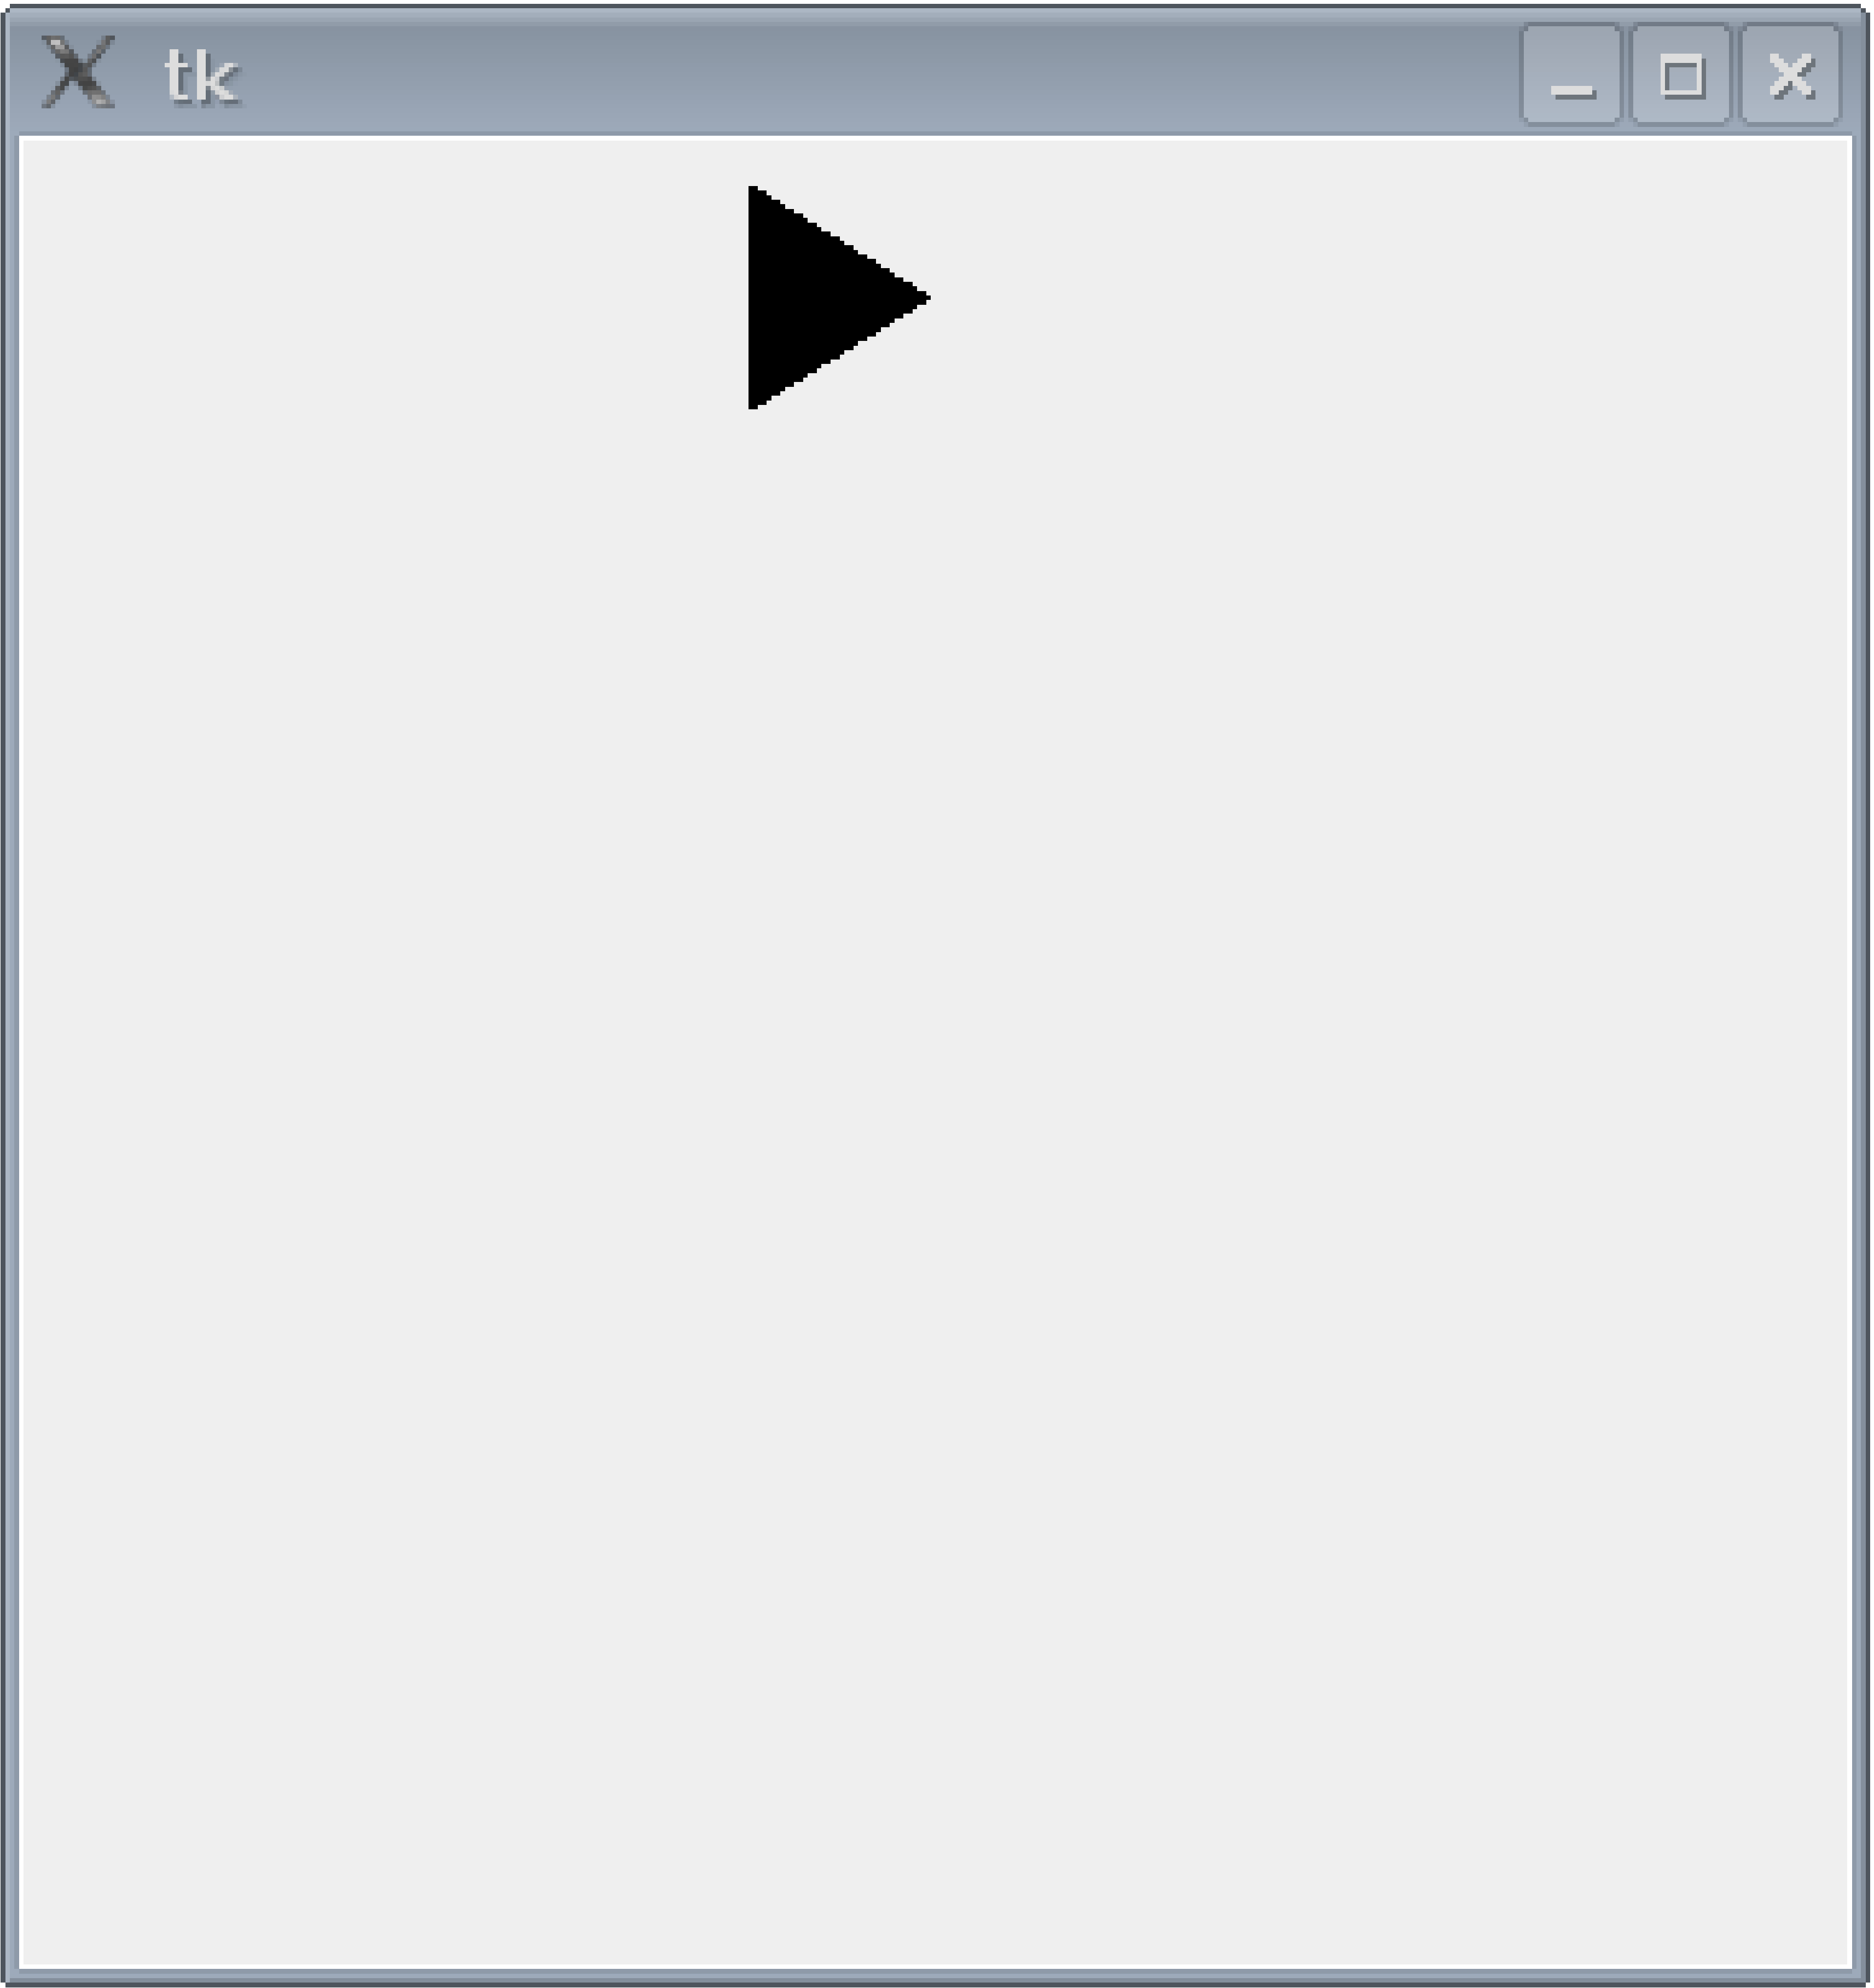
\includegraphics[width=80mm]{images/figure44}
\end{center}
\caption{Das Dreieck wandert über den Bildschirm.}\label{fig44}
\end{figure}

\par
%\emph{How does it work?}
\emph{Wie funktioniert das?}
\par
%Lines 1 to 5 we've seen before---it's just the basic setup to display a canvas---and in line 6, we create the triangle (using the \code{create\_polygon} function), and in line 7 you can see the identifier (the number 1) that is returned by this function. In line 8, we setup a simple for-loop to count from 0 to 59.
Zeile 1 bis 5 haben wir schon öfters so verwendet---wir stellen die Leinwand in einer bestimmten Größe dar---in Zeile 6 wird das Dreieck gezeichnet (mit der \code{create\_polygon} Funktion), und in Zeile 7 siehst du die eindeutige Nummer des Dreiecks (hier die Zahl 1), unter der das Dreieck aufrufbar ist. In Zeile 8 zählen wir in einer for-Schleife von 0 bis 40.

%The block of lines (9 to 11) is the code to move the triangle. The \code{move} function on the canvas object will move any drawn object by adding values to the object's x and y coordinates. For example, in line 9 we move the object with id 1 (the identifier for the triangle) 5 pixels across and 0 pixels down. If we wanted to move the back again we might use canvas.move(1, -5, 0)\index{modules!tkinter!move}.
Im Block der Zeilen 9 bis 11 wird das Dreieck bewegt. Die \code{move}-Funktion bewegt ein definiertes Objekt, indem es die x- und y-Koordinaten des Objektes verändert. In Zeile 9 bewegen wir das Objekt mit der Nummer 1 (also das Dreieck) um 5 Pixel nach rechts und 0 Pixel nach unten. Wenn wir es wieder zurück nach links bewegen wollten, müssten wir \code{leinwand.move(1, -5, 0)}\index{Module!tkinter!move} verwenden.

%The function \code{update} on the \code{tk} object forces it to update (if we didn't use \code{update}, tkinter would wait until the loop had finished before moving the triangle, which means you wouldn't see it move). Finally line 11 tells Python to sleep for 1/20th of a second (0.05), before continuing. We can change this code, so the triangle moves diagonally down the screen, by calling \code{move(1, 5, 5)}.  First, close the canvas (by clicking on the X button on the window), then try this code:
Die Funktion \code{tk.update} zeichnet das Dreieck in jedem Durchlauf der Schleife an die neue Position. Ansonsten würden wir die Bewegung nicht sehen. Und zu guter Letzt sagen wir Python in Zeile 11, dass Python eine zwanzigstel Sekunde (0.05) warten soll. Lass uns den Code so verändern, dass sich das Dreieck schräg nach unten bewegt. Mach zuerst die Leinwand zu, indem du auf die X-Schaltfläche am oberen Eck klickst. Probiere danach diesen Code:

%\begin{Verbatim}[frame=single]
%>>> import time
%>>> tk = Tk()
%>>> canvas = Canvas(tk, width=400, height=400)
%>>> canvas.pack()
%>>> canvas.create_polygon(10, 10, 10, 60, 50, 35)
%1
%>>> for x in range(0, 60):
%...     canvas.move(1, 5, 5)
%...     tk.update()
%...     time.sleep(0.05)
%...
%\end{Verbatim}
\begin{Verbatim}[frame=single]
>>> import time
>>> tk = Tk()
>>> leinwand = Canvas(tk, width=400, height=400)
>>> leinwand.pack()
>>> leinwand.create_polygon(10, 10, 10, 60, 50, 35)
1
>>> for x in range(0, 40):
...     leinwand.move(1, 5, 5)
...     tk.update()
...     time.sleep(0.05)
...
\end{Verbatim}

%Figure~\ref{fig45} shows the triangle part way down the screen. Move the triangle diagonally back up the screen to its starting position, by using -5, -5:
Abbildung~\ref{fig45} zeigt dir das Ergebnis der Bewegung. Wenn du das Dreieck wieder diogonal zurückbewegen willst, kannst du -5, -5 eingeben:

%\begin{Verbatim}[frame=single]
%>>> import time
%>>> for x in range(0, 60):
%...     canvas.move(1, -5, -5)
%...     tk.update()
%...     time.sleep(0.05)
%\end{Verbatim}
\begin{Verbatim}[frame=single]
>>> import time
>>> for x in range(0, 40):
...     leinwand.move(1, -5, -5)
...     tk.update()
...     time.sleep(0.05)
\end{Verbatim}

%\begin{figure}
%\begin{center}
%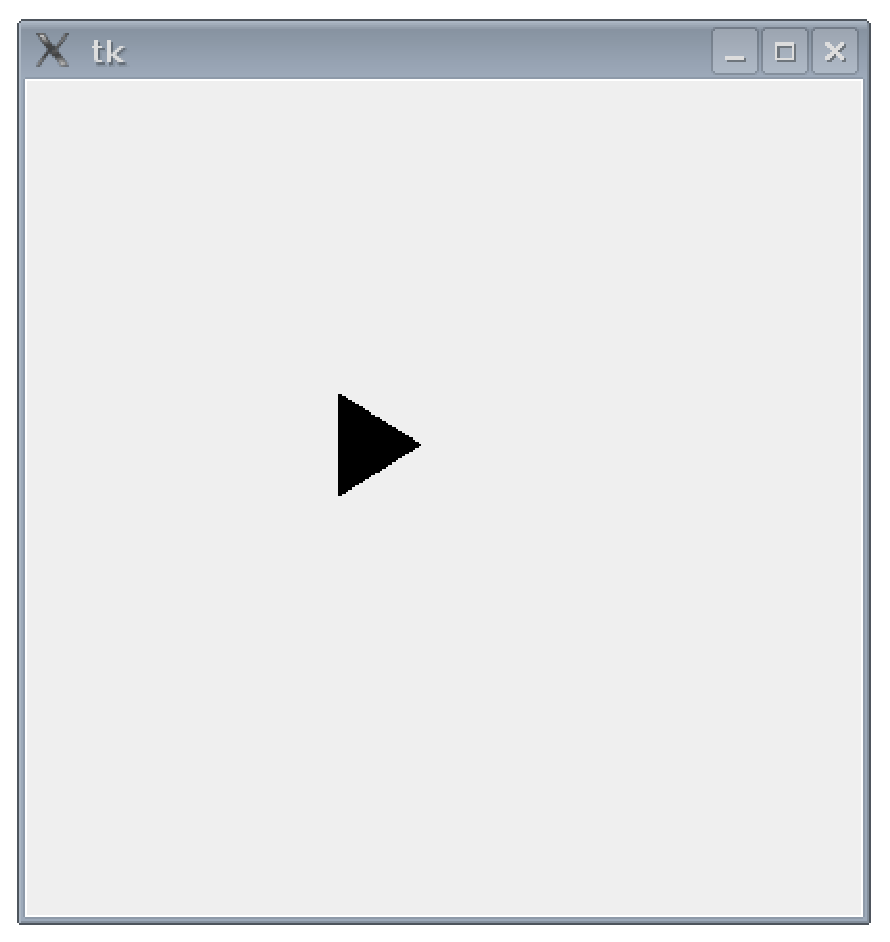
\includegraphics[width=80mm]{images/figure45}
%\end{center}
%\caption{The triangle moving down the screen.}\label{fig45}
%\end{figure}
\begin{figure}
\begin{center}
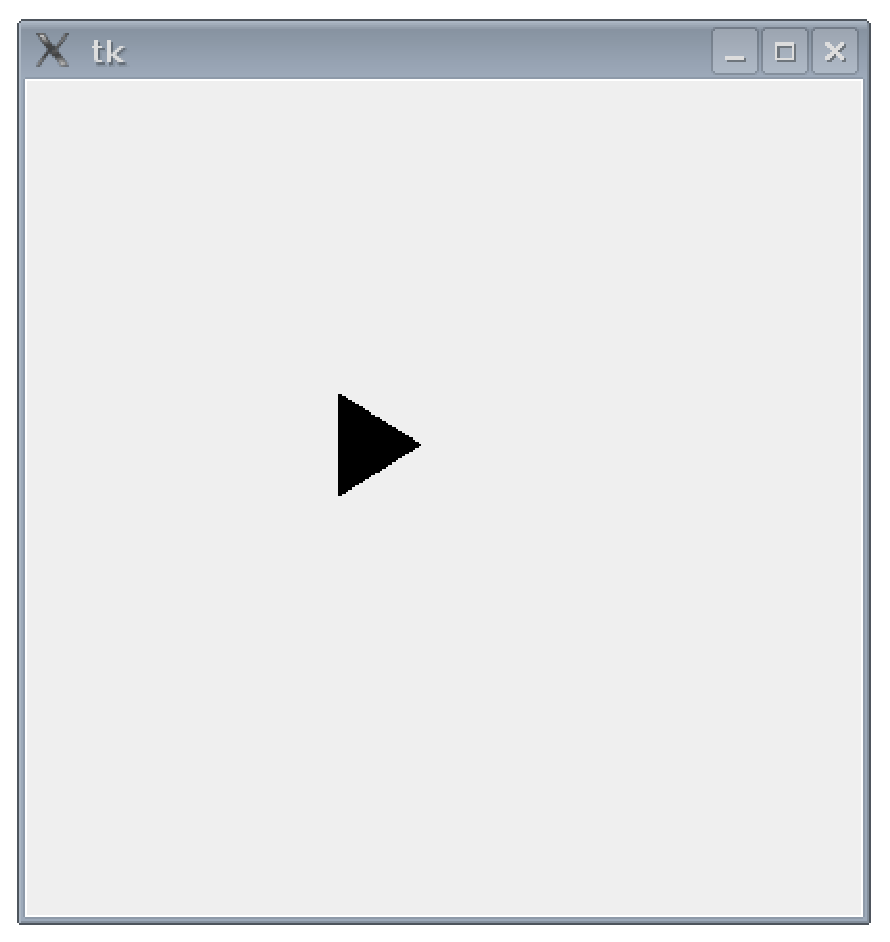
\includegraphics[width=80mm]{images/figure45}
\end{center}
\caption{Das Dreieck bewegt sich schräg nach unten.}\label{fig45}
\end{figure}

%\section{Reacting to events\texorpdfstring{$\ldots$}{...}}\index{modules!tkinter!events}
\section{Reagiere auf Ereignisse\texorpdfstring{$\ldots$}{...}}\index{Module!tkinter!events}

%We can also make the triangle react when someone hits a key, by using what are called \emph{event bindings}.  Events are things that occur while a program is running, such as someone moving the mouse, hitting a key, or even closing a window. You can setup \code{Tk} to look out for these events, and then do something in response. To begin handling events we need to start by creating a function. Suppose we want the triangle to move when the enter key is pressed? We can define a function to move the triangle:
Wir können das Dreieck auch mit der Tastatur steuern, indem wir sogenannte \emph{event bindings} verwenden. Ereignisse (engl. events) sind Dinge, die sich ereignen, während das Programm läuft. Also eine Mausbewegung oder ein Tastaturanschlag. Du kannst \code{Tk} so einstellen, dass es auf diese Ereignisse wartet und reagiert. Damit das also funktioniert, machen wir zuerst eine Funktion. Nehmen wir an, das Dreieck soll sich beim Drücken der Enter Taste bewegen. Also definieren wir eine Funktion um das Dreieck zu bewegen:

%\begin{Verbatim}[frame=single]
%>>> def movetriangle(event):
%...     canvas.move(1, 5, 0)
%\end{Verbatim}
\begin{Verbatim}[frame=single]
>>> def bewege_dreieck(ereignis):
...     leinwand.move(1, 5, 0)
\end{Verbatim}

%The function needs to have a single parameter (event), which is used by Tk to send information to the function about what has happened.  We then tell Tk that this function should be used for a particular event, using the \code{bind\_all}\index{modules!tkinter!bind\_all} function on the canvas. The full code looks like this:
Diese Funktion benötigt einen Parameter (ereignis), über den Tk Information an die Funktion sendet, was genau passiert ist. Zusätzlich sagen wir Tk, dass die Funktion immer bei einem bestimmten Ereignis aufgerufen werden soll, indem wir die \code{bind\_all}\index{Module!tkinter!bind\_all} Funktion mit der leinwand verbinden. Der Code schaut dann so aus:

%\begin{Verbatim}[frame=single]
%>>> from tkinter import *
%>>> tk = Tk()
%>>> canvas = Canvas(tk, width=400, height=400)
%>>> canvas.pack()
%>>> canvas.create_polygon(10, 10, 10, 60, 50, 35)
%>>> def movetriangle(event):
%...     canvas.move(1, 5, 0)
%...
%>>> canvas.bind_all('<KeyPress-Return>', movetriangle)
%\end{Verbatim}
\begin{Verbatim}[frame=single]
>>> from tkinter import *
>>> tk = Tk()
>>> leinwand = Canvas(tk, width=400, height=400)
>>> leinwand.pack()
>>> leinwand.create_polygon(10, 10, 10, 60, 50, 35)
>>> def bewege_dreieck(ereignis):
...     leinwand.move(1, 5, 0)
...
>>> leinwand.bind_all('<KeyPress-Return>', bewege_dreieck)
\end{Verbatim}

%The first parameter in the \code{bind\_all} function describes the event which we want Tk to look out for. In this case, it's the event \code{<KeyPress-Return>} (which is a press of the enter key).  We tell Tk that the \code{movetriangle} function should be called when this key-press event occurs.  If you run this code, click on the Tk canvas with your mouse, and then try hitting the Enter (or Return) key on your keyboard.
Der erste Parameter der \code{bind\_all} Funktion beschreibt die Ereignisse, auf die Tk warten soll. In diesem Fall ist es das Ereignis \code{<KeyPress-Return>} (also das Drücken der Enter-Taste). Dann sagen wir Tk, dass nach dem Drücken der Enter Taste die Funktion \code{bewege\_dreieck} aufgerufen werden soll. Wenn du diesen Code ausführst, klicke in das Bild mit dem Dreieck und drücke die Enter Taste auf der Tastatur.

%How about changing the direction of the triangle depending upon different key presses, such as the arrow keys? First of all we change the \code{move} triangle function to the following:
Wir könnten aber auch die Richtung der Bewegung mit den 4 Richtungstasten steuern. Zuerst ändern wir die \code{bewege\_dreieck}-Funktion:

%\begin{Verbatim}[frame=single]
%>>> def movetriangle(event):
%...     if event.keysym == 'Up':
%...         canvas.move(1, 0, -3)
%...     elif event.keysym == 'Down':
%...         canvas.move(1, 0, 3)
%...     elif event.keysym == 'Left':
%...         canvas.move(1, -3, 0)
%...     else:
%...         canvas.move(1, 3, 0)
%\end{Verbatim}
\begin{Verbatim}[frame=single]
>>> def bewege_dreieck(ereignis):
...     if ereignis.keysym == 'Up':
...         leinwand.move(1, 0, -3)
...     elif ereignis.keysym == 'Down':
...         leinwand.move(1, 0, 3)
...     elif ereignis.keysym == 'Left':
...         leinwand.move(1, -3, 0)
...     else:
...         leinwand.move(1, 3, 0)
\end{Verbatim}

%The event object that is passed to \code{movetriangle}, contains a number of \emph{properties}\footnote{Properties are named values, which describe something---for example, a property of the sky is that it's blue (sometimes), a property of a car is that it has wheels. In programming terms, a property has a name and a value.}.  One of these properties is \code{keysym}, which is a string holding the value of the actual key pressed.  If \code{keysym} contains the string `Up', we call \code{canvas.move} with the parameters (1, 0, -3); if it contains down we call with the parameters (1, 0, 3), and so on.  Remember that the first parameter is the identifying number for the shape drawn on the canvas, the second parameter is the value to add to the x (horizontal) coordinate, and the last parameter is the value to add to the y (vertical) coordinate. We then tell Tk that the \code{movetriangle} function should be used to handle events from 4 different keys (up, down, left and right).  So, the code now looks like this:
Das Objekt, welches von Tk an die Funktion \code{bewege\_dreieck} weitergegeben wird, enthält eine Anzahl von \emph{Eigenschaften}\footnote{Eigenschaften sind Werte, die etwas genauer beschreiben. Eine Eigenschaft von einem Auto ist zum Beispiel, dass es Räder hat. Eine Eigenschaft hat in Python einen Namen und einen Wert.}. Eine von diesen Eigenschaften it \code{keysym}, was ein String ist, in dem die aktuell gedrückte Taste verpackt ist. Wenn \code{keysym} den String `Up' enthält, rufen wir \code{bewege\_dreieck} mit den Parametern (1, 0, -3) auf; wenn es den Wert `Down' enthält, rufen wir die Funktion mit den Parametern (1, 0, 3) auf. Der erste Parameter ist immer die Nummer, die das Dreieck identifiziert, der zweite Parameter gibt an, wie weit nach rechts sich das Dreieck bewegen soll, und der dritte Parameter gibt an, wie weit nach unten. Zum Schluss müssen wir Tk noch sagen, auf alle 4 Tasten (links, rechts, oben, unten) zu reagieren. Also schaut der Code dann so aus:

%\begin{Verbatim}[frame=single]
%>>> from tkinter import *
%>>> tk = Tk()
%>>> canvas = Canvas(tk, width=400, height=400)
%>>> canvas.pack()
%>>> canvas.create_polygon(10, 10, 10, 60, 50, 35)
%1
%>>> def movetriangle(event):
%...     if event.keysym == 'Up':
%...         canvas.move(1, 0, -3)
%...     elif event.keysym == 'Down':
%...         canvas.move(1, 0, 3)
%...     elif event.keysym == 'Left':
%...         canvas.move(1, -3, 0)
%...     else:
%...         canvas.move(1, 3, 0)
%...
%>>> canvas.bind_all('<KeyPress-Up>', movetriangle)
%>>> canvas.bind_all('<KeyPress-Down>', movetriangle)
%>>> canvas.bind_all('<KeyPress-Left>', movetriangle)
%>>> canvas.bind_all('<KeyPress-Right>', movetriangle)
%\end{Verbatim}
\begin{Verbatim}[frame=single]
>>> from tkinter import *
>>> tk = Tk()
>>> leinwand = Canvas(tk, width=400, height=400)
>>> leinwand.pack()
>>> leinwand.create_polygon(10, 10, 10, 60, 50, 35)
1
>>> def bewege_dreieck(ereignis):
...     if ereignis.keysym == 'Up':
...         leinwand.move(1, 0, -3)
...     elif ereignis.keysym == 'Down':
...         leinwand.move(1, 0, 3)
...     elif ereignis.keysym == 'Left':
...         leinwand.move(1, -3, 0)
...     else:
...         leinwand.move(1, 3, 0)
...
>>> leinwand.bind_all('<KeyPress-Up>', bewege_dreieck)
>>> leinwand.bind_all('<KeyPress-Down>', bewege_dreieck)
>>> leinwand.bind_all('<KeyPress-Left>', bewege_dreieck)
>>> leinwand.bind_all('<KeyPress-Right>', bewege_dreieck)
\end{Verbatim}

\noindent
%With this example, the triangle now moves in the direction of the arrow key that you press.
Mit diesem Codebeispiel bewegt sich das Dreieck nun in die Richtung der gedrückten Pfeiltaste.

\newpage
